        %%******************************************%%
        %%                                          %%
        %%        Modello di tesi di laurea         %%
        %%            di Andrea Giraldin            %%
        %%                                          %%
        %%             2 novembre 2012              %%
        %%                                          %%
        %%******************************************%%


% I seguenti commenti speciali impostano:
% 1. 
% 2. PDFLaTeX come motore di composizione;
% 3. tesi.tex come documento principale;
% 4. il controllo ortografico italiano per l'editor.

% !TEX encoding = UTF-8
% !TEX TS-program = pdflatex
% !TEX root = tesi.tex
% !TEX spellcheck = it-IT

\documentclass[11pt,                    % corpo del font principale
               a4paper,                 % carta A4
               twoside,                 % impagina per fronte-retro
               openright,               % inizio capitoli a destra
               english,                 
               italian,                 
               ]{book}    

\usepackage[utf8]{inputenc}             % codifica di input; anche [latin1] va bene
                                        % NOTA BENE! va accordata con le preferenze dell'editor

%**************************************************************
% Importazione package
%************************************************************** 

%\usepackage{amsmath,amssymb,amsthm}    % matematica

\usepackage[english, italian]{babel}    % per scrivere in italiano e in inglese;
                                        % l'ultima lingua (l'italiano) risulta predefinita

\usepackage{bookmark}                   % segnalibri

\usepackage{caption}                    % didascalie

\usepackage{chngpage,calc}              % centra il frontespizio

\usepackage{csquotes}                   % gestisce automaticamente i caratteri (")

\usepackage{emptypage}                  % pagine vuote senza testatina e piede di pagina

\usepackage{epigraph}					% per epigrafi

\usepackage{eurosym}                    % simbolo dell'euro

\usepackage[T1]{fontenc}                % codifica dei font:
                                        % NOTA BENE! richiede una distribuzione *completa* di LaTeX

%\usepackage{indentfirst}               % rientra il primo paragrafo di ogni sezione

\usepackage{graphicx}                   % immagini

\usepackage{hyperref}                   % collegamenti ipertestuali



\usepackage[binding=5mm]{layaureo}      % margini ottimizzati per l'A4; rilegatura di 5 mm

\usepackage{listings}                   % codici

\usepackage{microtype}                  % microtipografia

\usepackage{mparhack,fixltx2e,relsize}  % finezze tipografiche

\usepackage{nameref}                    % visualizza nome dei riferimenti                                      

\usepackage[font=small]{quoting}        % citazioni

\usepackage{subfig}                     % sottofigure, sottotabelle

\usepackage[italian]{varioref}          % riferimenti completi della pagina

\usepackage[dvipsnames]{xcolor}         % colori

\usepackage{booktabs}                   % tabelle                                       
\usepackage{tabularx}                   % tabelle di larghezza prefissata                                    
\usepackage{longtable}                  % tabelle su più pagine                                        
\usepackage{ltxtable}                   % tabelle su più pagine e adattabili in larghezza

\usepackage[toc, acronym]{glossaries}   % glossario
                                        % per includerlo nel documento bisogna:
                                        % 1. compilare una prima volta tesi.tex;
                                        % 2. eseguire: makeindex -s tesi.ist -t tesi.glg -o tesi.gls tesi.glo
                                        % 3. eseguire: makeindex -s tesi.ist -t tesi.alg -o tesi.acr tesi.acn
                                        % 4. compilare due volte tesi.tex.

\usepackage[backend=biber,style=verbose-ibid,hyperref,backref]{biblatex}
                                        % eccellente pacchetto per la bibliografia; 
                                        % produce uno stile di citazione autore-anno; 
                                        % lo stile "numeric-comp" produce riferimenti numerici
                                        % per includerlo nel documento bisogna:
                                        % 1. compilare una prima volta tesi.tex;
                                        % 2. eseguire: biber tesi
                                        % 3. compilare ancora tesi.tex.

%**************************************************************
% file contenente le impostazioni della tesi
%**************************************************************

%**************************************************************
% Frontespizio
%**************************************************************
\newcommand{\myName}{Bogdan Ionut Suierica}                                    % autore
\newcommand{\myTitle}{Tres - Tree recommendation system}                    
\newcommand{\myDegree}{Tesi di laurea triennale}                % tipo di tesi
\newcommand{\myUni}{Università degli Studi di Padova}           % università
\newcommand{\myFaculty}{Corso di Laurea in Informatica}         % facoltà
\newcommand{\myDepartment}{Dipartimento di Matematica}          % dipartimento
\newcommand{\myProf}{Tullio Vardanega}                                % relatore
\newcommand{\myLocation}{Padova}                                % dove
\newcommand{\myAA}{2015-2016}                                   % anno accademico
\newcommand{\myTime}{Dec 2015}                                  % quando


%**************************************************************
% Impostazioni di impaginazione
% see: http://wwwcdf.pd.infn.it/AppuntiLinux/a2547.htm
%**************************************************************

\setlength{\parindent}{14pt}   % larghezza rientro della prima riga
\setlength{\parskip}{0pt}   % distanza tra i paragrafi


%**************************************************************
% Impostazioni di biblatex
%**************************************************************
\bibliography{bibliografia} % database di biblatex 

\defbibheading{bibliography}
{
    \cleardoublepage
    \phantomsection 
    \addcontentsline{toc}{chapter}{\bibname}
    \chapter*{\bibname\markboth{\bibname}{\bibname}}
}

\setlength\bibitemsep{1.5\itemsep} % spazio tra entry

\DeclareBibliographyCategory{opere}
\DeclareBibliographyCategory{web}

%\addtocategory{opere}{womak:lean-thinking}
\addtocategory{web}{site:agile-manifesto}

\defbibheading{opere}{\section*{Riferimenti bibliografici}}
\defbibheading{web}{\section*{Siti Web consultati}}


%**************************************************************
% Impostazioni di caption
%**************************************************************
\captionsetup{
    tableposition=top,
    figureposition=bottom,
    font=small,
    format=hang,
    labelfont=bf
}

%**************************************************************
% Impostazioni di glossaries
%**************************************************************

%**************************************************************
% Acronimi
%**************************************************************
\renewcommand{\acronymname}{Acronimi e abbreviazioni}

\newacronym[description={\glslink{apig}{Application Program Interface}}]
    {api}{API}{Application Program Interface}

\newacronym[description={\glslink{umlg}{Unified Modeling Language}}]
    {uml}{UML}{Unified Modeling Language}
    
\newacronym[description={\glslink{ictg}{Information and Communications Technology}}]
	{ict}{ICT}{Information and Communications Technology}
	
\newacronym[description={\glslink{cmsg}{Content Management System}}]
{cms}{CMS}{Content Management System}

\newacronym[description={\glslink{mvcg}{Model-View-Controller}}]
{mvc}{MVC}{Model-View-Controller}

\newacronym[description={\glslink{ideg}{Integrated Development Environment}}]
{IDE}{IDE}{Integrated Development Environment}

\newacronym[description={\glslink{restg}{Representational State Transfer}}]
{REST}{REST}{Representational State Transfer}

\newacronym[description={\glslink{urig}{Uniform Resource Identifier}}]
{URI}{URI}{Uniform Resource Identifier}

\newacronym[description={\glslink{jsong}{Javascript Object Notation}}]
{JSON}{JSON}{Javascript Object Notation}

\newacronym[description={\glslink{jvmg}{Java Virtual Machine}}]
{JVM}{JVM}{Java Virtual Machine}

\newacronym[description={\glslink{daog}{Data Access Object}}]
{dao}{DAO}{Data Access Object}

\newacronym[description={\glslink{pdca}{Plan-Do-Check-Act}}]
{pdca}{PDCA}{Plan-Do-Check-Act}


%**************************************************************
% Glossario
%**************************************************************
%\renewcommand{\glossaryname}{Glossario}

\newglossaryentry{gantt}
{
	name=\glslink{gantt}{Gantt},
	text=Gantt,
	sort=gantt,
	description={Il diagramma di Gantt è uno strumento di supporto alla gestione dei progetti che permette la rappresentazione grafica di un calendario di attività. Esso è utile al fine di pianificare, coordinare e tracciare specifiche attività in un progetto dandone una chiara illustrazione dello stato d'avanzamento.}
}

\newglossaryentry{slack}
{
	name=\glslink{slack}{Slack},
	text=slack,
	sort=slack,
	description={periodo di inattività.}
}

\newglossaryentry{singleton}
{
	name=\glslink{singleton}{Singleton},
	text=Singleton,
	sort=Singleton,
	description={è un design pattern creazionale che ha lo scopo di garantire che di una determinata classe venga creata una e una sola istanza, e di fornire un punto di accesso globale a tale istanza.}
}

\newglossaryentry{strategy}
{
	name=\glslink{strategy}{Strategy},
	text=Strategy,
	sort=Strategy,
	description={è uno dei pattern comportamentali. Viene utilizzato per definire una famiglia di algoritmi, incapsularli e renderli intercambiabili (in base ad una qualche condizione) in modo trasparente al client che ne fa uso. Il pattern è utile in quelle situazioni dove sia necessario modificare dinamicamente gli algoritmi utilizzati da un'applicazione.}
}

\newglossaryentry{daog}
{
	name=\glslink{dao}{DAO},
	text=Data Access Object,
	sort=dao,
	description={è un pattern architetturale per la gestione della persistenza: si tratta fondamentalmente di una classe con relativi metodi che rappresenta un'entità tabellare di un RDBMS, usata principalmente in applicazioni web, per stratificare e isolare l'accesso ad una tabella/record tramite query (poste all'interno dei metodi della classe) ovvero al data layer da parte della business logic creando un maggiore livello di astrazione ed una più facile manutenibilità. I metodi del DAO con le rispettive query dentro verranno così richiamati dalle classi della business logic.}
}

\newglossaryentry{repository}
{
	name=\glslink{repository}{Repository},
	text=repository,
	sort=repository,
	description={database in grado di contenere svariate tipologie di dati, corredate da relative informazioni (metadati). Offre inoltre un sistema di versionamento in grado di tener traccia delle modifiche effettuate al suo interno.}
}

\newglossaryentry{jvmg}
{
	name=\glslink{JVM}{JVM},
	text=JVM,
	sort=JVM,
	description={è la componente della piattaforma Java che esegue i programmi tradotti in bytecode dopo una prima compilazione}
}

\newglossaryentry{jsong}
{
	name=\glslink{JSON}{JSON},
	text=JSON,
	sort=JSON,
	description={è un formato adatto per lo scambio dei dati in applicazioni client-server}
}

\newglossaryentry{urig}
{
	name=\glslink{URI}{URI},
	text=URI,
	sort=URI,
	description={la locuzione Uniform Resource Identifier in informatica, si riferisce a una stringa che identifica univocamente una risorsa generica che può essere un indirizzo Web, un documento, un’immagine, un file, un servizio, un indirizzo di posta elettronica, ecc..}
}

\newglossaryentry{restg}
{
	name=\glslink{REST}{REST},
	text=REST,
	sort=REST,
	description={un tipo di architettura software per i sistemi di ipertesto distribuiti come il World Wide Web}
}

\newglossaryentry{ideg}
{
	name=\glslink{IDE}{IDE},
	text=IDE,
	sort=IDE,
	description={software che, in fase di programmazione, aiuta i programmatori nello sviluppo del codice sorgente di un programma. Spesso aiuta lo sviluppatore segnalando errori di sintassi del codice direttamente in fase di scrittura, oltre a tutta una serie di strumenti e funzionalità di supporto alla fase di sviluppo e debugging}
}

\newglossaryentry{git}
{
	name=\glslink{git}{Git},
	text=git,
	sort=git,
	description={sistema software di controllo versione}
}

\newglossaryentry{framework}
{
	name=\glslink{framework}{Framework},
	text=framework,
	sort=framework,
	description={in informatica, e specificatamente nello sviluppo software, un framework è un'architettura logica di supporto su cui un software può essere progettato e realizzato, spesso facilitandone lo sviluppo da parte del programmatore}
}

\newglossaryentry{mvcg}
{
	name=\glslink{mvc}{MVC},
	text=Model-View-Controller,
	sort=mvc,
	description={il Model-View-Controller, in informatica, è un pattern architetturale molto diffuso nello sviluppo di sistemi software, in particolare nell'ambito della programmazione orientata agli oggetti, in grado di separare la logica di presentazione dei dati dalla logica di business}
}

\newglossaryentry{cmsg}
{
	name=\glslink{cms}{CMS},
	text=Content Management System,
	sort=cms,
	description={strumento software installato su un server web studiato per facilitare la gestione dei contenuti dei siti web, svincolando l'amministratore da conoscenze tecniche di programmazione}
}

\newglossaryentry{ictg}
{
	name=\glslink{ict}{ICT},
	text=Information and Communications Technology,
	sort=ict,
	description={l'insieme dei metodi e delle tecnologie che realizzano i sistemi di trasmissione, ricezione ed elaborazione di informazioni (tecnologie digitali comprese)}
}

\newglossaryentry{apig}
{
    name=\glslink{api}{API},
    text=Application Program Interface,
    sort=api,
    description={in informatica con il termine \emph{Application Programming Interface API} (ing. interfaccia di programmazione di un'applicazione) si indica ogni insieme di procedure disponibili al programmatore, di solito raggruppate a formare un set di strumenti specifici per l'espletamento di un determinato compito all'interno di un certo programma. La finalità è ottenere un'astrazione, di solito tra l'hardware e il programmatore o tra software a basso e quello ad alto livello semplificando così il lavoro di programmazione}
}

\newglossaryentry{umlg}
{
    name=\glslink{uml}{UML},
    text=UML,
    sort=uml,
    description={in ingegneria del software \emph{UML, Unified Modeling Language} (ing. linguaggio di modellazione unificato) è un linguaggio di modellazione e specifica basato sul paradigma object-oriented. L'\emph{UML} svolge un'importantissima funzione di ``lingua franca'' nella comunità della progettazione e programmazione a oggetti. Gran parte della letteratura di settore usa tale linguaggio per descrivere soluzioni analitiche e progettuali in modo sintetico e comprensibile a un vasto pubblico}
}

 % database di termini
\makeglossaries


%**************************************************************
% Impostazioni di graphicx
%**************************************************************
\graphicspath{{immagini/}} % cartella dove sono riposte le immagini


%**************************************************************
% Impostazioni di hyperref
%**************************************************************
\hypersetup{
    %hyperfootnotes=false,
    %pdfpagelabels,
    %draft,	% = elimina tutti i link (utile per stampe in bianco e nero)
    colorlinks=true,
    linktocpage=true,
    pdfstartpage=1,
    pdfstartview=FitV,
    % decommenta la riga seguente per avere link in nero (per esempio per la stampa in bianco e nero)
    %colorlinks=false, linktocpage=false, pdfborder={0 0 0}, pdfstartpage=1, pdfstartview=FitV,
    breaklinks=true,
    pdfpagemode=UseNone,
    pageanchor=true,
    pdfpagemode=UseOutlines,
    plainpages=false,
    bookmarksnumbered,
    bookmarksopen=true,
    bookmarksopenlevel=1,
    hypertexnames=true,
    pdfhighlight=/O,
    %nesting=true,
    %frenchlinks,
    urlcolor=webbrown,
    linkcolor=RoyalBlue,
    citecolor=webgreen,
    %pagecolor=RoyalBlue,
    %urlcolor=Black, linkcolor=Black, citecolor=Black, %pagecolor=Black,
    pdftitle={\myTitle},
    pdfauthor={\textcopyright\ \myName, \myUni, \myFaculty},
    pdfsubject={},
    pdfkeywords={},
    pdfcreator={pdfLaTeX},
    pdfproducer={LaTeX}
}

%**************************************************************
% Impostazioni di itemize
%**************************************************************
\renewcommand{\labelitemi}{$\ast$}

%\renewcommand{\labelitemi}{$\bullet$}
%\renewcommand{\labelitemii}{$\cdot$}
%\renewcommand{\labelitemiii}{$\diamond$}
%\renewcommand{\labelitemiv}{$\ast$}


%**************************************************************
% Impostazioni di listings
%**************************************************************
\lstset{
    language=[LaTeX]Tex,%C++,
    keywordstyle=\color{RoyalBlue}, %\bfseries,
    basicstyle=\small\ttfamily,
    %identifierstyle=\color{NavyBlue},
    commentstyle=\color{Green}\ttfamily,
    stringstyle=\rmfamily,
    numbers=none, %left,%
    numberstyle=\scriptsize, %\tiny
    stepnumber=5,
    numbersep=8pt,
    showstringspaces=false,
    breaklines=true,
    frameround=ftff,
    frame=single
} 


%**************************************************************
% Impostazioni di xcolor
%**************************************************************
\definecolor{webgreen}{rgb}{0,.5,0}
\definecolor{webbrown}{rgb}{.6,0,0}


%**************************************************************
% Altro
%**************************************************************

\newcommand{\omissis}{[\dots\negthinspace]} % produce [...]

% eccezioni all'algoritmo di sillabazione
\hyphenation
{
    ma-cro-istru-zio-ne
    gi-ral-din
}

\newcommand{\sectionname}{sezione}
\addto\captionsitalian{\renewcommand{\figurename}{figura}
                       \renewcommand{\tablename}{tabella}}

\newcommand{\glsfirstoccur}{\ap{{[g]}}}

\newcommand{\intro}[1]{\emph{\textsf{#1}}}

%**************************************************************
% Environment per ``rischi''
%**************************************************************
\newcounter{riskcounter}                % define a counter
\setcounter{riskcounter}{0}             % set the counter to some initial value

%%%% Parameters
% #1: Title
\newenvironment{risk}[1]{
    \refstepcounter{riskcounter}        % increment counter
    \par \noindent                      % start new paragraph
    \textbf{\arabic{riskcounter}. #1}   % display the title before the 
                                        % content of the environment is displayed 
}{
    \par\medskip
}

\newcommand{\riskname}{Rischio}

\newcommand{\riskdescription}[1]{\textbf{\\Descrizione:} #1.}

\newcommand{\risksolution}[1]{\textbf{\\Soluzione:} #1.}

%**************************************************************
% Environment per ``use case''
%**************************************************************
\newcounter{usecasecounter}             % define a counter
\setcounter{usecasecounter}{0}          % set the counter to some initial value

%%%% Parameters
% #1: ID
% #2: Nome
\newenvironment{usecase}[2]{
    \renewcommand{\theusecasecounter}{\usecasename #1}  % this is where the display of 
                                                        % the counter is overwritten/modified
    \refstepcounter{usecasecounter}             % increment counter
    \vspace{10pt}
    \par \noindent                              % start new paragraph
    {\large \textbf{\usecasename #1: #2}}       % display the title before the 
                                                % content of the environment is displayed 
    \medskip
}{
    \medskip
}

\newcommand{\usecasename}{UC}

\newcommand{\usecaseactors}[1]{\textbf{\\Attori Principali:} #1. \vspace{4pt}}
\newcommand{\usecasepre}[1]{\textbf{\\Precondizioni:} #1. \vspace{4pt}}
\newcommand{\usecasedesc}[1]{\textbf{\\Descrizione:} #1. \vspace{4pt}}
\newcommand{\usecasepost}[1]{\textbf{\\Postcondizioni:} #1. \vspace{4pt}}
\newcommand{\usecasealt}[1]{\textbf{\\Scenario Alternativo:} #1. \vspace{4pt}}

%**************************************************************
% Environment per ``namespace description''
%**************************************************************

\newenvironment{namespacedesc}{
    \vspace{10pt}
    \par \noindent                              % start new paragraph
    \begin{description} 
}{
    \end{description}
    \medskip
}

\newcommand{\classdesc}[2]{\item[\textbf{#1:}] #2}                     % file con le impostazioni personali

\begin{document}
%**************************************************************
% Materiale iniziale
%**************************************************************
\frontmatter
% !TEX encoding = UTF-8
% !TEX TS-program = pdflatex
% !TEX root = ../tesi.tex
% !TEX spellcheck = it-IT

%**************************************************************
% Frontespizio 
%**************************************************************
\begin{titlepage}

\begin{center}

\begin{LARGE}
\textbf{\myUni}\\
\end{LARGE}

\vspace{10pt}

\begin{Large}
\textsc{\myDepartment}\\
\end{Large}

\vspace{10pt}

\begin{large}
\textsc{\myFaculty}\\
\end{large}

\vspace{30pt}
\begin{figure}[htbp]
\begin{center}

\includegraphics[height=6cm]{logo-unipd}
\end{center}
\end{figure}
\vspace{30pt} 

\begin{LARGE}
\begin{center}
\textbf{\myTitle}\\
\end{center}
\end{LARGE}

\vspace{10pt} 

\begin{large}
\textsl{\myDegree}\\
\end{large}

\vspace{40pt} 

\begin{large}
\begin{flushleft}
\textit{Relatore}\\ 
\vspace{5pt} 
Prof. \myProf
\end{flushleft}

\vspace{0pt} 

\begin{flushright}
\textit{Laureando}\\ 
\vspace{5pt} 
\myName
\end{flushright}
\end{large}

\vspace{40pt}

\line(1, 0){338} \\
\begin{normalsize}
\textsc{Anno Accademico \myAA}
\end{normalsize}

\end{center}
\end{titlepage} 
% !TEX encoding = UTF-8
% !TEX TS-program = pdflatex
% !TEX root = ../tesi.tex
% !TEX spellcheck = it-IT

%**************************************************************
% Colophon
%**************************************************************
\clearpage
\phantomsection
\thispagestyle{empty}

\hfill

\vfill

\noindent\myName: \textit{\myTitle,}
\myDegree,
\textcopyright\ \myTime.
% !TEX encoding = UTF-8
% !TEX TS-program = pdflatex
% !TEX root = ../tesi.tex
% !TEX spellcheck = it-IT

%**************************************************************
% Dedica
%**************************************************************
\cleardoublepage
\phantomsection
\thispagestyle{empty}
\pdfbookmark{Dedica}{Dedica}

\vspace*{3cm}

%\begin{center}
%Lorem ipsum dolor sit amet, consectetuer adipiscing elit. \\ \medskip
%--- Oscar Wilde    
%\end{center}

\medskip

\begin{center}
\textit{Dedicato ai miei genitori, senza i quali non avrei mai potuto raggiungere questo traguardo, a mia sorella Adina ed a Gabi.}\\
\end{center}

% !TEX encoding = UTF-8
% !TEX TS-program = pdflatex
% !TEX root = ../tesi.tex
% !TEX spellcheck = it-IT

%**************************************************************
% Sommario
%**************************************************************
\cleardoublepage
\phantomsection
\pdfbookmark{Sommario}{Sommario}
\begingroup
\let\clearpage\relax
\let\cleardoublepage\relax
\let\cleardoublepage\relax

\chapter*{Sommario}

Il presente documento descrive il lavoro svolto dal laureando Bogdan Ionut Suierica, durante il periodo di stage, della durata di circa trecentoventi ore, presso l'azienda Nextep S.r.l., con sede a Carmignano di Brenta(PD). Si andranno a descrivere dettagliatamente le attività svolte durante il tirocinio e si analizzeranno i risultati ottenuti. Il progetto, caratterizzante lo stage, consisteva nella realizzazione di un motore di raccomandazioni, in linguaggio Scala, attraverso l'utilizzo del \gls{framework} Play. L'obiettivo era utilizzare l'algoritmo Id3 per introdurre un albero decisionale, grafo di decisioni e delle loro possibile conseguenze, con l'intenzione di creare un 'piano di azioni' mirato ad un scopo, ovvero la raccomandazione finale.
Il presente documento ha lo scopo di illustrare la panoramica dell'azienda dove è stato svolto lo stage, le attività svolte, e di fornire in conclusione una valutazione personale.

\chapter*{Note}
Per evitare qualsiasi dubbio e per permettere una maggiore chiarezza e comprensione del testo su termini ambigui, abbreviazioni e acronimi utilizzati, è presente il glossario in appendice. I termini tecnici e quelli in lingua straniera sono dati in \textit{corsivo}.

%\vfill
%
%\selectlanguage{english}
%\pdfbookmark{Abstract}{Abstract}
%\chapter*{Abstract}
%
%\selectlanguage{italian}

\endgroup			

\vfill


%% !TEX encoding = UTF-8
% !TEX TS-program = pdflatex
% !TEX root = ../tesi.tex
% !TEX spellcheck = it-IT

%**************************************************************
% Ringraziamenti
%**************************************************************

\cleardoublepage
\phantomsection
\pdfbookmark{Ringraziamenti}{ringraziamenti}

\begin{flushright}{
	\slshape    
	``Life is really simple, but we insist on making it complicated''} \\ 
	\medskip
    --- Confucius
\end{flushright}


\bigskip

\begingroup
\let\clearpage\relax
\let\cleardoublepage\relax
\let\cleardoublepage\relax

%
\chapter*{Ringraziamenti}

\noindent \textit{Innanzitutto, vorrei esprimere la mia gratitudine al Prof. NomeDelProfessore, relatore della mia tesi, per l'aiuto e il sostegno fornitomi durante la stesura del lavoro.}\\

\noindent \textit{Desidero ringraziare con affetto i miei genitori per il sostegno, il grande aiuto e per essermi stati vicini in ogni momento durante gli anni di studio.}\\

\noindent \textit{Ho desiderio di ringraziare poi i miei amici per tutti i bellissimi anni passati insieme e le mille avventure vissute.}\\
\bigskip

\noindent\textit{\myLocation, \myTime}
\hfill \myName
%
\endgroup


% !TEX encoding = UTF-8
% !TEX TS-program = pdflatex
% !TEX root = ../tesi.tex
% !TEX spellcheck = it-IT

%**************************************************************
% Indici
%**************************************************************
\cleardoublepage
\pdfbookmark{\contentsname}{tableofcontents}
\setcounter{tocdepth}{2}
\tableofcontents
%\markboth{\contentsname}{\contentsname} 
\clearpage

\begingroup 
    \let\clearpage\relax
    \let\cleardoublepage\relax
    \let\cleardoublepage\relax
    %*******************************************************
    % Elenco delle figure
    %*******************************************************    
    \phantomsection
    \pdfbookmark{\listfigurename}{lof}
    \listoffigures

    \vspace*{8ex}

    %*******************************************************
    % Elenco delle tabelle
    %*******************************************************
    \phantomsection
    \pdfbookmark{\listtablename}{lot}
    \listoftables
        
    \vspace*{8ex}
\endgroup

\cleardoublepage

\cleardoublepage

%**************************************************************
% Materiale principale
%**************************************************************
\mainmatter
% !TEX encoding = UTF-8
% !TEX TS-program = pdflatex
% !TEX root = ../tesi.tex
% !TEX spellcheck = it-IT

%**************************************************************
\chapter{Profilo Aziendale}
\label{cap:introduzione}
%**************************************************************

Lo stage formativo, oggetto del presente elaborato, è stato da me svolto presso l'azienda Nextep S.r.l.\footnote{\url{http://www.nextep.it/}}, con sede a Carmignano di Brenta (PD). Nextep S.r.l. è una società fondata nel 2000 che opera nel settore dell'informatica e della comunicazione. Il \textit{core business} è riconosciuto nelle attività di progettazione, realizzazione e gestione di infrastrutture di \textit{Information e Digital Communication Technology.}\\
L'azienda è suddivisa in due divisioni principali:
\begin{itemize}
	\item \textbf{Divisione \textit{marketing} e commerciale}: si occupa di studiare il mercato e la clientela;
	\item \textbf{Divisione tecnica}: si occupa della gestione e la realizzazione dei progetti.
\end{itemize}

\begin{figure}[h]
\centering
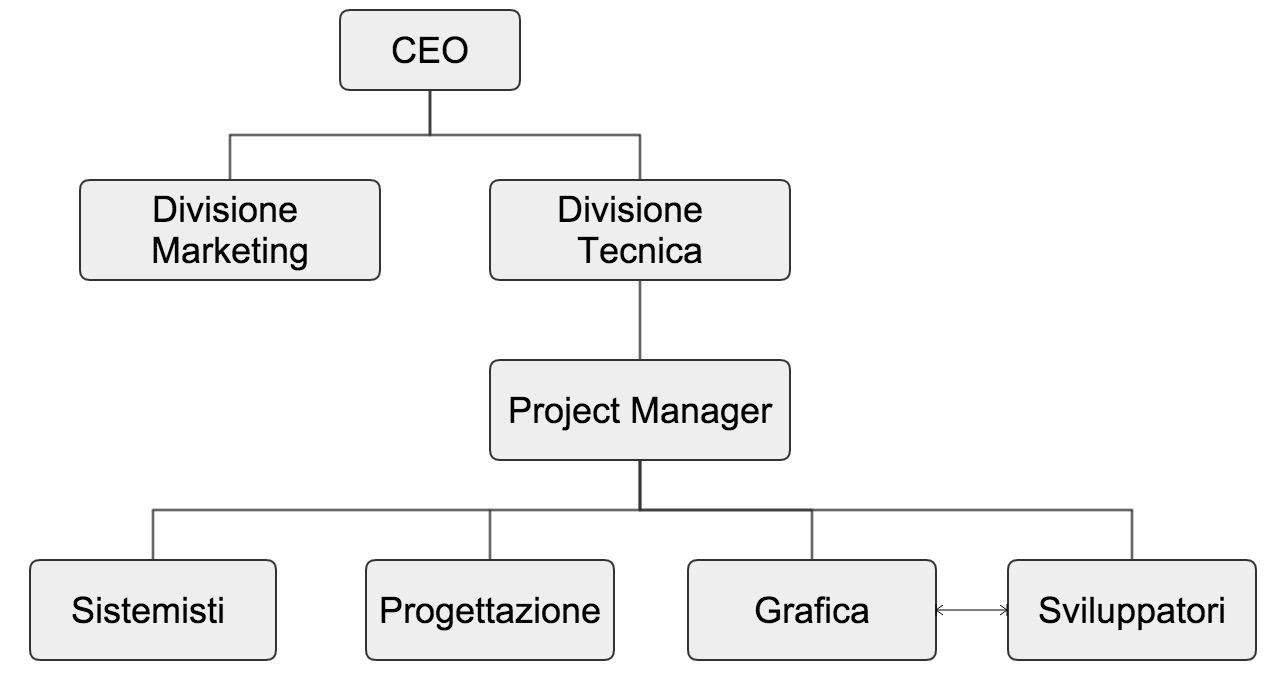
\includegraphics[width=0.8\linewidth]{immagini/organigramma}
\caption[Organigramma dell'azienda]{Organigramma dell'azienda}
\label{fig:logo-nextep}
\end{figure}

L'organico di Nextep S.r.l. è formato da circa 20 persone, suddivisi tra grafici, sviluppatori, \textit{marketing} e sistemisti. L'azienda fa parte del gruppo Allos\footnote{\url{http://www.allos.it/}} che insieme a Zero12\footnote{\url{http://www.zero12.it/}} condividono l'ambiente di lavoro. Il risultato è un ambiente di \textit{coworking} dove si condividono esperienze e conoscenze. Non è raro che le tre aziende collaborino tra di loro per la realizzazione di alcuni progetti.


%**************************************************************
\section{Prodotti e servizi offerti}

L'azienda offre soluzioni innovative che permettono ai cliente di affrontare il mercato con una marcia tecnologica in più, legata sia all'innovazione di prodotto che ai processi interni di pianificazione e produzione.

%**************************************************************
\subsection{Prodotti}

Il settore principale di Nextep S.r.l. è il web. Nello specifico l'azienda si occupa di:
\begin{itemize}
	\item Progettazione e sviluppo di siti web e portali;
	\item Progettazione e sviluppo di \textit{Social Intranet }e capitalizzazione della cultura aziendale;
	\item Progettazione e sviluppo di soluzioni \textit{e-commerce};
	\item Progettazione e realizzazione di applicazioni \textit{mobile};
	\item Studio e progettazione della grafica /\textit{user experience};
	\item Integrazione con tecnologie e servizi di \textit{cloud computing};
	\item Analisi, ideazione e realizzazione di azioni di \textit{web markenting}.
\end{itemize}

\begin{figure}[h]
\centering
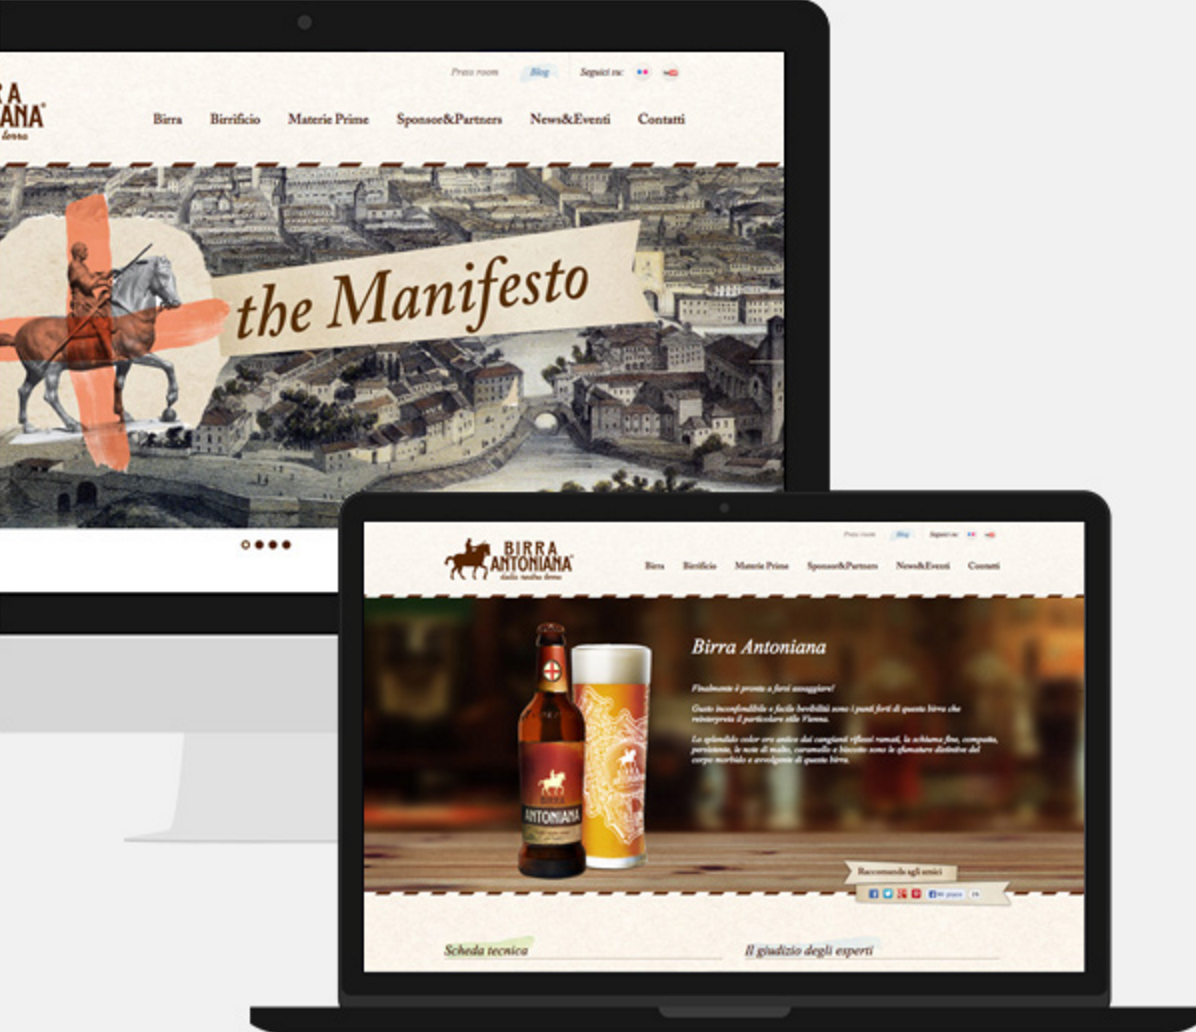
\includegraphics[width=0.5\linewidth]{immagini/sito}
\caption[Birra Antoniana: uno dei siti realizzati da Nextep]{Birra Antoniana: uno dei siti realizzati da Nextep}
\label{fig:sito}
\end{figure}
L'azienda offre un sevizio innovativo di \textit{web design}, marketing e grafica, visibile su tutte le piattaforme e su tutti i dispositivi, quali \textit{smartphone} e \textit{tablet} . Propone interfacce semplici per la gestione dei contenuti e un design evoluto e personalizzato, fornendo soluzioni diverse a seconda delle necessità dei clienti.


%**************************************************************
\subsection{Servizi}

I principali servizi offerti da \textbf{Nextep S.r.l. }ai propri clienti sono:
\begin{itemize}
	\item Fornitura di servizi a canone (server virtuali, applicazioni web, servizi di \textit{monitoring }di infrastrutture \gls{ict}, \textit{backup-online}, canoni di assistenza e manutenzione dei sistemi, canoni di gestione dei sistemi);
	\item Elaborazione dati, analisi e supporto decisionale in ambito \textit{web marketing, social marketing e social intranet};
	\item Consulenza e formazione di \textit{web marketing, social marketing, web analytics};
	\item Servizio Clienti, attività di supporto tecnico e di gestione di infrastrutture \gls{ict} e siti web.
\end{itemize}

\section{Tecnologia di riferimento}
Le tecnologie maggiormente utilizzate per lo sviluppo dei progetti sono le seguenti:
\begin{itemize}
	\item \textbf{Linguaggi di programmazione: }
	\begin{itemize}
		\item \textbf{Php: }il più utilizzato per la realizzazione dei \textit{Web-service};
		\item \textbf{Java, Scala: }utilizzati per le \textit{Web-application};
		\item \textbf{HTML, CSS, Javascript: }utilizzati per la scrittura di pagine web.
	\end{itemize}
	\item \textbf{Framework e CMS: }per facilitare lo sviluppo e il riutilizzo del codice delle proprie applicazioni Nextep S.r.l. utilizza vari \gls{framework} e \gls{cms}:
	\begin{itemize}
		\item \textbf{Play: }web \gls{framework} scritto in Scala. Permette di scrivere applicativi web sia in linguaggio Java che Scala. Segue il \textit{pattern }\gls{mvc};
		\item \textbf{Bootstrap: }si tratta del \gls{framework} \textit{front-end }più utilizzato. Permette di scrivere pagine \textit{web responsive};
		\item \textbf{Compass: }\gls{framework} che fornisce delle estensioni CSS3. Permette di organizzare il CSS in maniera migliore ed aumentare la facilità di manutenzione;
		\item \textbf{Drupal: }il più popolare \gls{cms} PHP. Permette di avere un riutilizzo sistematico del codice scritto e quindi di ridurre i tempi di sviluppo e manutenzione.
	\end{itemize}
	\item \textbf{Database: }il database viene scelto, tenendo conto dei vantaggi/svantaggi di ognuno dei database elencati sotto:
	\begin{itemize}
		\item \textbf{OrientDB: }è un multi-model \textit{No-Sql }\textit{database }scritto in Java;
		\item \textbf{MongoDB: }\textit{database} \textit{NO-SQL}, particolarmente adatto quando vengono gestite grandi quantità di dati;
		\item \textbf{MySQL, SQL Server, PostGreeSQL }: \textit{database }\textit{SQL}.
	\end{itemize}
\end{itemize}
\begin{figure}[h]
\centering
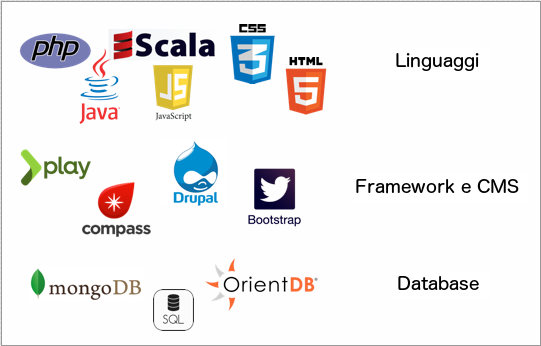
\includegraphics[width=0.6\linewidth]{immagini/White}
\caption[Classificazione delle tecnologie utilizzate]{Classificazione delle tecnologie utilizzate}
\label{fig:White}
\end{figure}

\newpage
\section{Processi aziendali}
\subsection{Metodologia agile}
L'azienda utilizza una gestione dei progetti seguendo un metodo \textit{agile}\footnote{\url{http://agilemanifesto.org/}}, in quanto, proprio per la particolarità del servizio offerto, è più importante mantenere una costante collaborazione con il cliente, rendendolo partecipe del progetto e mostrando così una rapida reattività alle nuove richieste. I principi su cui si basa il modello di tipo \textit{agile} sono:
\begin{itemize}
	\item Gli individui  e le iterazione rispetto ai processi  e agli strumenti;
	\item Software funzionante rispetto ad un'ampia documentazione;
	\item Committenti e sviluppatori devono lavorare insieme per tutta la durata del progetto;
	\item La pronta risposta ai cambiamenti rispetto all'esecuzione di un piano.
\end{itemize}

\begin{figure}[h]
\centering
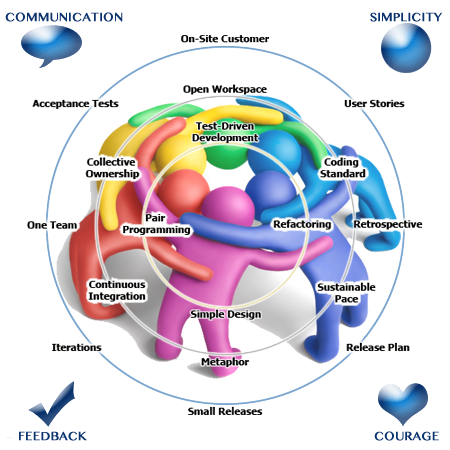
\includegraphics[width=0.55\linewidth]{immagini/agile}
\caption[Raffigurazione della metodologia agile]{Raffigurazione della metodologia agile. L'immagine in figura è tratta da \href{https://github.com/emccode/training}{Emccode}}
\label{fig:agile}
\end{figure}
Nello specifico il team di sviluppo segue un approccio \textit{Scrum}\footnote{\url{https://it.wikipedia.org/wiki/Scrum_(informatica)}} per i progetti più complessi. Questo modello è basato sui seguenti concetti:
\begin{itemize}
	\item \textbf{Sprint: }unità base dello sviluppo \textit{Scrum }. Durante uno \textit{sprint }non è possibile modificare gli obiettivi precedentemente pianificati;
	\item\textbf{Riunioni: }
	\begin{itemize}
		\item Prima dello \textit{sprint } le riunioni costituiscono il momento di pianificazione degli obiettivi e della durata dello sprint;
		\item Dopo lo \textit{sprint} costituiscono il momento di verifica del lavoro svolto;
		\item Quotidianamente;
		\item Riunioni con i clienti per capire a fondo i requisiti richiesti.
	\end{itemize}
	\item \textbf{Product Backlog: }rappresenta ciò che deve essere fatto in una lista ordinata di requisiti relativi ad un prodotto software, ognuno dei quali avente una priorità;
	\item \textbf{Sprint Backlog: }lista del lavoro che deve essere effettuato nel corso dello \textit{sprint }successivo;
	\item \textbf{Incremento: }è la somma di tutti gli elementi del \textit{Product Backlog }completati duranti gli \textit{sprint} precedenti;
	\item \textbf{Burn down: }è la rappresentazione grafica del lavoro da svolgere, in base al tempo che si ha a disposizione.
\end{itemize}

\begin{figure}[h]
\centering
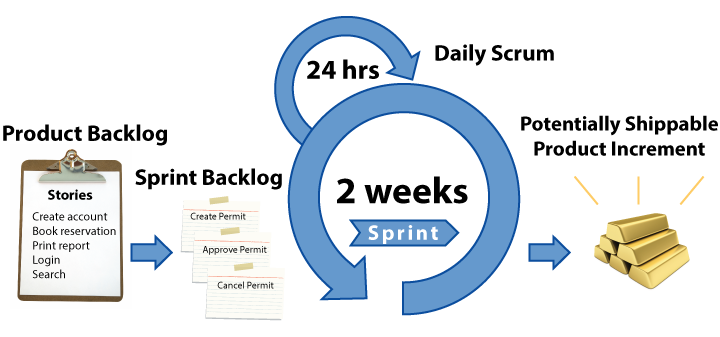
\includegraphics[width=0.8\linewidth]{immagini/scrum}
\caption[Una panoramica su scrum]{Una panoramica su scrum. L'immagine in figura è tratta dall'\href{http://www.agilenutshell.com/scrum}{articolo "\textit{Agile In a Nutshell}"}}
\label{fig:scrum}
\end{figure}


Non essendo un gruppo molto ampio, questo modello si adatta bene all'azienda, che può così diventare flessibile e reagire velocemente ai cambiamenti dei requisiti che si verificano durante lo sviluppo software.

\subsection{Strumenti a supporto dei processi}
\subsection*{Gestione di progetto}
Nextep utilizza \textit{Zendesk}\footnote{\url{https://www.zendesk.it/}} per fornire assistenza ai clienti attraverso diversi canali, tra cui \textit{email, telefono, chat, web e social media}. Tutte le iterazioni su \textit{Zendesk} sono tracciate fornendo dati importanti dell'azienda così come un'analisi della \textit{performance} individuale. In questo modo si ha una visione globale sull'andamento del progetto.
\begin{figure}[h]
\centering
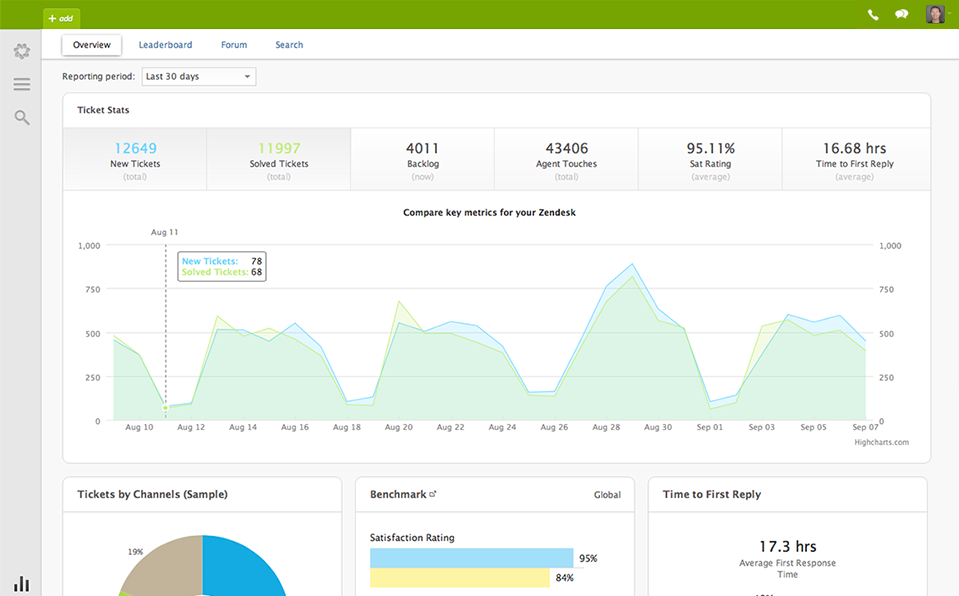
\includegraphics[width=1.1\linewidth]{immagini/reporting}
\caption[Esempio Report Zendesk]{Esempio Report Zendesk}
\label{fig:reporting}
\end{figure}

Per la gestione del progetto viene utilizzato \textit{Jira Agile}\footnote{\url{https://jira.atlassian.com/secure/Dashboard.jspa}} seguendo il modello delle \textit{user story}. \textit{Jira} è un tool per la pianificazione, organizzazione e verifica del lavoro. Esso permette di:
\begin{itemize}
	\item Gestire e assegnare \textit{ticket};
	\item Integrare i progetti con il sistema di versionamento \gls{git}\footnote{\url{http://git-scm.com/}};
	\item Pianificare le attività;
	\item Gestione dei \textit{task }e delle ore di lavoro.
\end{itemize}

\subsection*{Scrum board}
Una \textit{scrum board }è una lavagna fisica o virtuale per la gestione delle varie attività del processo produttivo. Essa suddivide in colonne i vari stati evolutivi del prodotto. Ogni colonna può contenere diversi \textit{post-it} che rappresentano un determinato \textit{task}. Uno spostamento rappresenta un'evoluzione o una regressione. Questo strumento viene utilizzato dal team di sviluppo per la gestione della produzione e per avere un panorama dello stato di avanzamento dei lavori. I \textit{post-it} vengono inseriti dai \textit{project manager} e ogni colore ha una priorità diversa, in base a una legenda conosciuta dall'intero team. \\
La suddivisione degli stati della \textit{Scrum board }è la seguente:

\begin{figure}[h]
\centering
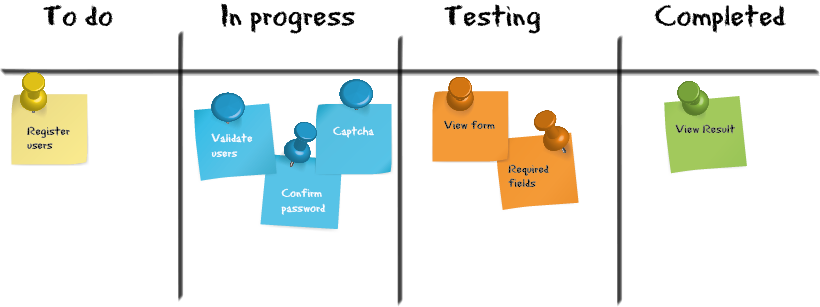
\includegraphics[width=1\linewidth]{immagini/scrum-board}
\caption[Scrum board]{Scrum board}
\label{fig:scrum-board}
\end{figure}

\begin{itemize}
	\item \textbf{To Do: }detto anche \textit{backlog }rappresenta un prodotto appena commissionato che deve essere ancora assegnato;
	\item \textbf{In progress: }indica che l'attività è stata presa in carico ed è in fase di sviluppo;
	\item \textbf{Testing: }indica la terminazione dello sviluppo e l'inizio della fase di \textit{testing};
	\item \textbf{Completed: }il prodotto finito è stato approvato.
\end{itemize}

\subsection*{Documentazione}
Per la realizzazione dei documenti inerenti ai progetti viene utilizzato \textit{Google Docs}. In questo modo si permette a più dipendenti di collaborare allo stesso documento, anche contemporaneamente, essendo accessibile a tutti attraverso il \textit{browser}. È possibile utilizzare la cronologia delle revisioni per conoscere le vecchie versioni e l'autore di ogni modifica.

\subsection*{Sistema di versionamento}
Come sistema di versionamento Nextep S.r.l. utilizza \gls{git}.\\
I \gls{repository} dei progetti si trovano su dei server gestiti dai dipendenti dell'azienda.

\subsection*{Ambiente di sviluppo}
L'ambiente di sviluppo varia a seconda delle tecnologie coinvolte nel progetto proposto.\\
Vengono utilizzati i seguenti \gls{IDE}:
\begin{itemize}
	\item \textbf{Eclipse/IntelliJ: }per lo sviluppo di applicazioni in Java/Scala;
	\item \textbf{Smultron/PhpStorm: }per lo sviluppo di applicazioni in Php;
	\item \textbf{Sublime Text: }per lo sviluppo di codice HTML/CSS/Javascript e Php.
\end{itemize}

\subsection*{Sistemi operativi}
Nextep S.r.l. non impone nessun obbligo sul sistema operativo utilizzato. All'interno dell'azienda i dipendenti utilizzano vari sistemi operativi come \textit{Windows, Linux e Mac OS}, in base alla propria preferenza.\\
Durante l'ultima settimana di permanenza nell'azienda, sono venuto a conoscenza dell'acquisto di vari computer \textit{Mac Book e iMac }per permettere, a chiunque lo desidera, di passare o effettuare l'\textit{upgrade }al nuovo \textit{OS X}.\\
I \textit{server }utilizzati per il \textit{deployment }sono solitamente macchine con sistema operativo \textit{Linux Ubuntu} o \textit{Linux Debian} residenti in \textit{Amazon Web Services (AWS).}

\begin{figure}[h]
\centering
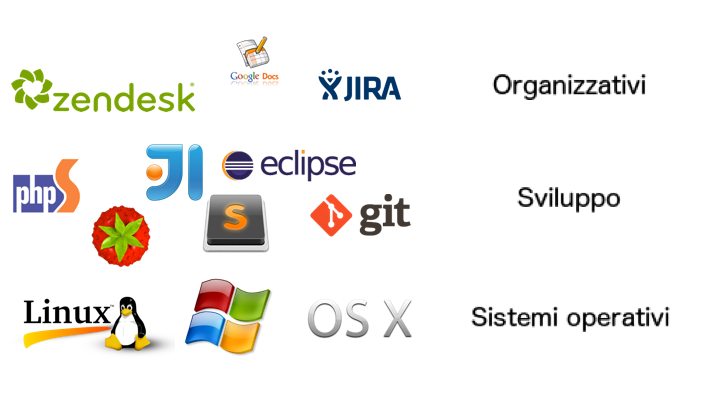
\includegraphics[width=0.7\linewidth]{immagini/gestione}
\caption[Classificazione degli strumenti utilizzati]{Classificazione degli strumenti utilizzati}
\label{fig:gestione}
\end{figure}

\section{Tipologia di clientela e propensione all'innovazione}
L'azienda offre i propri servizi a diverse tipologie di clientela: dalle piccole aziende e i singoli professionisti, alle medie e grandi aziende. I principali clienti sono aziende italiane del settore \textit{retail}, manifatturiero e \textit{corporate}. \\
Per l'azienda è importante innovare per restare competitiva e acquisire e/o mantenere una posizione importante sul mercato, specialmente lavorando nell'ambito del Web. In tal senso, Nextep S.r.l. sta cercando persone che abbiano un'attitudine positiva verso il cambiamento. Anche lo spazio di \textit{coworking} in cui ha sede Nextep S.r.l. è luogo di condivisione, un vero e proprio laboratorio di innovazione, promossa dalle tre aziende. Oltre alle riunioni e ai vantaggi offerti dall'ambiente di lavoro appena descritto, l'azienda svolge dei corsi di formazione del personale con lo scopo di mantenere coinvolto e motivato l'intero \textit{team}.             % Profilo Aziendale
% !TEX encoding = UTF-8
% !TEX TS-program = pdflatex
% !TEX root = ../tesi.tex
% !TEX spellcheck = it-IT

%**************************************************************
\chapter{Il progetto nella strategia aziendale}
\label{cap:processi-metodologie}
%**************************************************************

\intro{Questo capitolo intende fornire una descrizione dettagliata del progetto di stage e dei motivi che hanno spinto l'azienda a proporlo oltre che i benefici derivati da tale progetto. Nel capitolo discuto anche i vincoli tecnologici e metodologici che l'azienda ha imposto sul mio stage}\\

%**************************************************************
\section{Presentazione del progetto}
Il progetto di stage riguarda la realizzazione di un motore di raccomandazione basato sul guadagno informativo negli alberi decisionali. Il sistema deve consentire il salvataggio del comportamento dell'utente, all'interno di un sito, e costruire un albero attraverso la classificazione dell'appartenenza di un oggetto ad una classe (immagini cliccata o non cliccata, \textit{hover}, ecc.). Questo tipo di apprendimento deve funzionare anche per gli esempi non ancora forniti al sistema: solamente dall'osservazione di fatti e oggetti relativi all'ambiente circostante, il sistema deve generalizzare i dati e le informazioni ricevute, ottenendo conoscenza che, auspicalmente, sia valida anche per i casi non ancora osservati.\\
Un albero decisionale è un piano strutturato ad albero che individua una successione di test sugli attributi noti e cioè il comportamento dell'utente al fine di predire un attributo  di output e cioè la raccomandazione. Prima della creazione dell'albero bisogna stabilire quali test effettuare su quali attributi. Ad ogni passo della creazione dell'albero, l'algoritmo deve scegliere su quale attributo fare lo \textit{split}.\\
Ad esempio un albero decisionale per decidere  se è la giornata ideale per giocare a tennis è il seguente:
\begin{figure}[h]
\centering
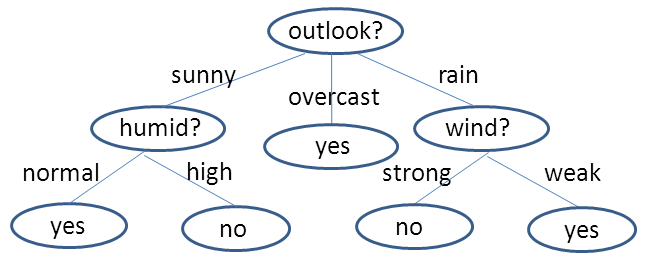
\includegraphics[width=0.7\linewidth]{immagini/play}
\caption[Esempio di albero decisionale]{Esempio di albero decisionale}
\label{fig:albero-decisionale-esempio}
\end{figure}

\newpage
\subsection{Obiettivi dello stage}
Lo stage ha una durata prevista di 300-320 ore complessive. Prima dell'inizio dello stage, \textbf{Nextep }ha redatto il \textit{Piano di Lavoro }contenente tutti gli obiettivi da realizzare nelle settimane di stage.
Gli obiettivi dello stage erano suddivisi in obiettivi minimi e obiettivi massimi. Durante le settimane  di lavoro essi hanno subito delle modifiche dovute alla strategia aziendale e dalle priorità del team di sviluppo. In un primo momento, infatti, è stato fatto il \textit{porting }da \textit{MongoDB a OrientDB }e l'\textit{upgrade }di versione del \gls{framework} Play di un progetto preesistente chiamato DRE. Questo ha comportato un ritardo di quanto pianificato e il lavoro è stato sospeso per realizzare il nuovo modulo Tres.\\
Di seguito sono riportati gli obiettivi dello stage:
\begin{itemize}
	\item \textbf{Obiettivi formativi:}
	\begin{itemize}
		\item Formazione sui sistemi di raccomandazione e degli algoritmi di apprendimento;
		\item Studio delle tecnologie utilizzate, Scala e OrientDB;
		\item Studio degli strumenti utilizzati, in particolar modo del \gls{framework} e degli \gls{IDE}.
	\end{itemize}
	\item \textbf{Obiettivi minimi:}
	\begin{itemize}
		\item Utilizzo del \textit{database} OrientDB.
	\end{itemize}
	\item \textbf{Obiettivi massimi:}
	\begin{itemize}
		\item Implementazioni di nuovi modelli di algoritmi di apprendimento per migliorare l'individuazione dei gusti dell'utente;
		\item Migliorare la fase di apprendimento del modello stesso;
		\item Implementazioni di algoritmi di \textit{cluster }per il raggruppamento di elementi omogenei in un insieme di dati.
	\end{itemize}
\end{itemize}

\subsection{Motivazioni}
La motivazione che spinge l'azienda a investire sugli stagisti è la possibilità di entrare in un settore di mercato differente dalle loro attività principali. Con lo scopo di capire se l'idea è utile e vantaggiosa, si creano le opportunità di stage durante i quali gli stagisti si prendono l'impegno di sviluppare un prodotto con le funzionalità attese dall'azienda; tuttavia non è escluso un possibile inserimento nel proprio organico dello stagista, infatti, l'azienda, attraverso l'attivazione di tirocini, avrà la possibilità di individuare, di valutare e di formare i futuri soggetti da inserire all'interno dell'azienda, superando quella che è la fase più dispendiosa.\\
Il progetto di stage rientra in una strategia aziendale che punta a rilasciare nuove funzionalità per i progetti attivi. In particolare si è costatato che una grande parte delle attività era la gestione di notevoli quantità di dati. Ciò rende il problema della gestione e dell'organizzazione di questa mole informativa una questione quantomai prioritaria, che cerca soluzioni nuove e facilitano l'esperienza utente. \textit{Nextep} vuole sfruttare questi dati e fornire un servizio di raccomandazione attraverso la classificazione del comportamento dell'utente, con l'aiuto di un albero decisionale, all'interno di un sito. Con il rilascio, l'azienda vuole fornire un servizio di tipo \textit{Software as a service} (SaaS), attraverso il quale fornirà all'utente la possibilità di gestire autonomamente i contenuti.\\
L'obiettivo principale dello stage consta nel realizzare un prototipo del prodotto.

\section{Vincoli di progetto}

\subsection{Vincoli del dominio}
Il sistema da realizzare deve riuscire a gestire una grande quantità di dati e l'architettura deve permettere di scalare facilmente e deve avere un'alta affidabilità. Per questo viene usato OrientDB come \textit{database} nella sua versione a grafo. Un database a grafo è simile a una struttura a rete composto da nodi e spigoli. OrientDB permette di scalare il database all'aumentare dei dati attraverso lo \textit{sharding}, usando \textit{cluster} multipli per classe, in cui ogni \textit{cluster} ha una propria lista di \textit{server} dove replicare i dati.
\begin{figure}[h]
\centering
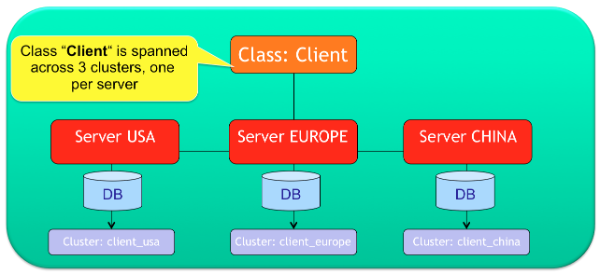
\includegraphics[width=0.9\linewidth]{immagini/distributed-sharding-class}
\caption[Esempio classe "Client" diviso in 3 clusters]{Esempio classe "Client" diviso in 3 \textit{clusters}. Questa immagine è stata presa dalla documentazione ufficiale di \href{http://orientdb.com/docs/last/Distributed-Sharding.html}{OrientDB}}
\label{fig:distributed-sharding-class}
\end{figure}

\subsection{Vincoli tecnologici}
\subsubsection*{Play framework}
Per lo sviluppo dell'applicativo è stato utilizzato il \gls{framework} Play\footnote{\url{https://www.playframework.com/documentation/2.4.x/Home}}. Esso è scritto in Scala e permette lo sviluppo delle \textit{web application} concorrenti, distribuite e altamente scalabili. \\
Play consente di ottimizzare lo sviluppo permettendo di ricaricare le classi modificate senza dover riavviare il server, ma solamente ricaricando le pagine dal \textit{browser}.\\
Le caratteristiche principali di Play sono:
\begin{itemize}
	\item Permette la visualizzazione degli errori direttamente dal \textit{browser};
	\item Utilizza il \textit{design pattern} \gls{mvc}\footnote{\url{https://www.playframework.com/documentation/1.0/main}};
	\item Possiede un motore di \textit{template} per le pagine HTML in linguaggio Scala;
	\item Rende facile la realizzazione di servizi \gls{REST}. \gls{REST} utilizza un aggregato di dati con un nome(\gls{URI}) e una rappresentazione, in questo caso \gls{JSON}, su cui è possibile invocare operazioni \textit{CREATE, READ, UPDATE, DELETE} (CRUD). Le associazioni tra richieste e \textit{controller} sono tutte mappate all'interno del file \textit{route} presente in tutti i progetti Play;
	\item Fornisce delle classi per facilitare la manipolazione di oggetti \gls{JSON};
	\item Permette di gestire facilmente le dipendenze verso librerie esterne sviluppate da terzi attraverso il file SBT\footnote{\url{http://www.scala-sbt.org/index.html}} contenente tutte le dipendenze del progetto;
	\item Fornisce librerie per realizzare i test su quanto sviluppato.\footnote{\url{https://www.playframework.com/documentation/2.0/ScalaTest}}
\end{itemize}
Tutte le richieste HTTP vengono gestite da Play nel modo seguente:
\begin{itemize}
	\item Il \gls{framework} riceve la richiesta HTTP;
	\item Viene cercato nel file \textit{route} l'azione del \textit{controller} corrispondente alla richiesta;
	\item Il codice del \textit{controller} viene eseguito;
	\item Se necessario il \textit{controller} genera una \textit{view} da ritornare al chiamante;
	\item Il \textit{controller} restituisce una risposta HTTP.
\end{itemize}
\begin{figure}[h]
\centering
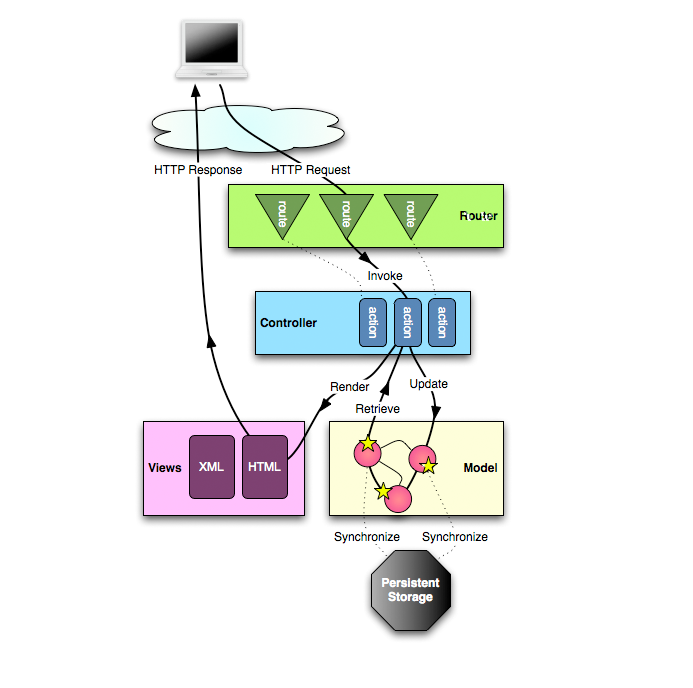
\includegraphics[width=0.8\linewidth]{immagini/diagrams_path}
\caption[Gestione di una richiesta HTTP in Play]{Gestione di una richiesta HTTP in Play. Questa immagine è stata presa dalla documentazione ufficiale di \href{https://www.playframework.com/documentation/1.0/main}{\textit{Play Framework}}}
\label{fig:diagrams_path}
\end{figure}

\newpage
\subsection*{OrientDB}
Come DBMS per il salvataggio dei dati si è scelto di utilizzare OrientDB\footnote{\url{http://orientdb.com/}}, nella sua versione di tipo \textit{graphdatabase}. Riesce a modellare ogni tipo di dominio, anche complesso, come un grafo, dove ogni entità è un \textit{Vertex},vertice in italiano, e tutte le relazioni sono \textit{Edge}, spigoli.
\begin{figure}[h]
\centering
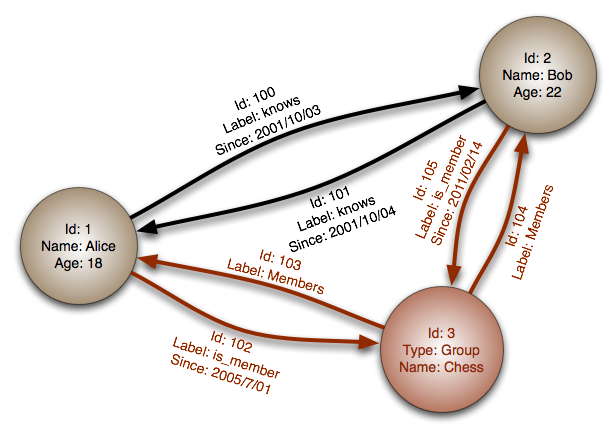
\includegraphics[width=0.8\linewidth]{immagini/GraphDatabase_PropertyGraph}
\caption[Esempio modellazione in OrientDB]{Esempio modellazione in OrientDB. Questa immagine è stata presa dall'\href{https://en.wikipedia.org/wiki/Graph_database}{articolo sui \textit{database} a graffo di Wikipedia}}
\label{fig:GraphDatabase_PropertyGraph}
\end{figure}

Le caratteristiche chiave di OrientDB sono:
\begin{itemize}
	\item Multiple modalità di \textit{storage: document, graph}(con supporto allo \textit{stack} Tinkerpop\footnote{\url{http://tinkerpop.incubator.apache.org/}}), \textit{object, key/value};
	\item Funzionamento \textit{embedded, in memory, client/server};
	\item Fornisce le proprietà ACID (Atomicità, Coerenza, Isolamento e Durabilità) di consistenza delle transizioni;
	\item Supporta nativamente \gls{JSON} e \gls{REST};
	\item È scritto in Java e quindi può girare su moltissime piattaforme.
\end{itemize}
Le caratteristiche che hanno portato alla scelta di OrientDB sono:
\begin{itemize}
	\item \textbf{Niente più join}: si può utilizzare il concetto di oggetti embedded ma supporta anche le relazioni senza l'uso del costoso \textit{JOIN}. Al contrario OrientDB usa i puntatori tra \textit{records}. Nella seguente immagine si può osservare la relazione tra due \textit{record} usando l'id \#8:124 per connettere \textit{Order} con \textit{Customer}.
	\begin{figure}[h]
	\centering
	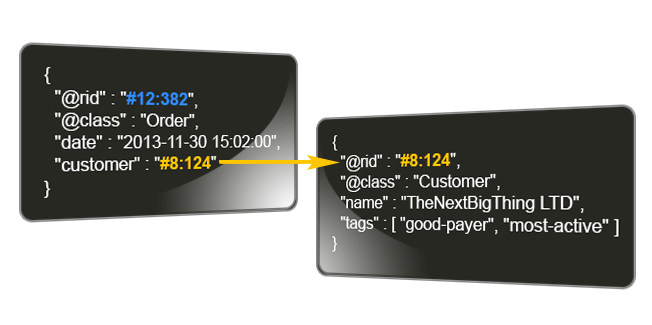
\includegraphics[width=0.8\linewidth]{immagini/json_linked3}
	\caption[Relazione tra due documenti]{Relazione tra due documenti. Questa immagine è stata presa dal sito ufficiale di \href{http://orientdb.com/orientdb-vs-mongodb/}{OrientDB}}
	\label{fig:json_linked3}
	\end{figure}
	

\item \textbf{Pensato per i big data}: con i database relazionali e documentali, più dati abbiamo, più lento diventa. OrientDB gestisce le relazioni come dei \textit{link} fisici ai \textit{records}. Questi vengono assegnati un'unica volta alla creazione del \textit{Edge} in tempo O(1);
\item \textbf{Scalabile:} OrientDB è un database scalabile. All'aumentare della dimensione del \textit{database} è possibile suddividere i dati del db in parti dette \textit{shard}, semplicemente aggiungendo un nodo nella rete che sarà automaticamente accettato dal \textit{server} distribuito senza bisogno di configurazioni. Le sincronizzazioni saranno automatiche non appena il \textit{server} sarà online;
\begin{figure}[h]
\centering
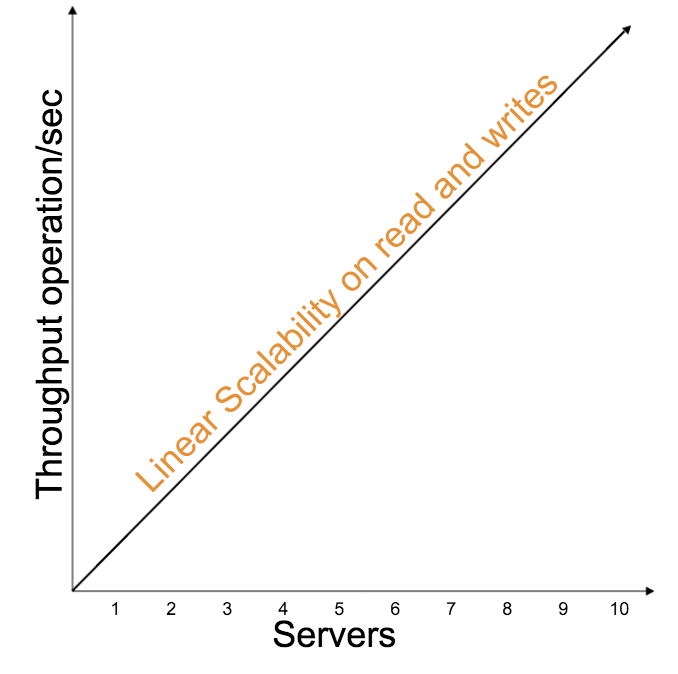
\includegraphics[width=0.7\linewidth]{immagini/rapporto-scalabilita}
\caption[Rapporto scalabilità]{Rapporto scalabilità}
\label{fig:rapporto-scalabilità}
\end{figure}


\item \textbf{Ripristino dati in caso di crash:} grazie a WAL (\textit{Write Ahead Logging}), OrientDB è capace di ripristinare il contenuto del database in caso di \textit{crash}. Tutte le transazioni in pendenza tornano allo stato in cui erano prima che le modifiche venissero apportate e tutti i cliente connessi al nodo vengono automaticamente spostati su un nodo \textit{server} disponibile.
\end{itemize}
La versione utilizzata durante lo stage è \textit{"orientdb-community-2.1.5"}. Per interagire con il \textit{database} si è scelto di utilizzare le Java \gls{api} nella versione \textit{graph} \gls{api}.

\subsection*{Scala}
Il linguaggio di programmazione scelto per lo sviluppo è Scala\footnote{\url{http://www.scala-lang.org/}}. È un linguaggio per la \gls{JVM} staticamente tipato, a paradigma misto. Cerca di unire la programmazione ad oggetti con la programmazione funzionale, permettendo a seconda della situazione, di scegliere l'approccio più adatto a soddisfare le esigenze.  Scala semplifica certi problemi di progettazione, in particolare quelli legati alla concorrenza. I linguaggi funzionali \textit{"puri"} non permettono alcun stato mutabile, evitando di conseguenza il bisogno di sincronizzazione sull'accesso condiviso allo stato mutabile. Invece, i programmi scritti in linguaggi puramente funzionali comunicano scambiando messaggi tra processi autonomi e concorrenti. Scala supporta questo modello con la sua libreria di attori, ma consente di usare variabili mutabili e immutabili.\\
Le funzioni sono cittadini \textit{"di prima classe"} nella programmazione funzionale, nel senso che possono essere assegnate a variabili, passate ad altre funzioni, esattamente come gli altri valori. Questa caratteristica promuove la composizione di comportamenti avanzati usando operazioni primitive. Dato che Scala aderisce al principio per cui ogni cosa è un oggetto, in Scala anche le funzioni sono oggetti.\\ Il linguaggio ha una sintassi molto concisa e sintetica rispetto ad altri linguaggio e permette di ridurre drasticamente il numero di linee di codice necessarie ma il codice scritto non è di facile lettura.

\subsection{Vincoli metodologici}
Lo strumento di versionamento scelto durante lo sviluppo è Git\footnote{\url{https://git-scm.com/}}. Il motivo decisivo nella scelta di questa strumento è stata l'esperienza acquisita durante il corso di Ingegneria del Software.\\
Per la realizzazione dei diagrammi \gls{uml} durante le varie attività dello stage formativo è stato scelto di utilizzare Astah Professional\footnote{\url{http://astah.net/editions/professional}} perchè:
\begin{itemize}
	\item Possiedo una \textit{student license};
	\item È lo stesso strumento utilizzato durante il corso di \textit{Ingegneria del Software};
	\item Aderisce allo standard \gls{uml} 2.0.	
\end{itemize}
L'\gls{IDE} scelto è stato Intellij IDEA\footnote{\url{https://www.jetbrains.com/idea/}}. I motivi che hanno portato a questa scelta sono:
\begin{itemize}
	\item Offre la miglior integrazione con il linguaggio Scala ed il \gls{framework} Play;
	\item Permette di avviare e stoppare il \textit{server} direttamente da interfaccia grafica;
	\item Permette di utilizzare il terminale direttamente di Intellij IDEA;
	\item È un software molto leggere in confronto agli altri come Eclipse.
\end{itemize}
Per realizzare la documentazione del codice sorgente è stato utilizzato ScalaDoc\footnote{\url{http://docs.scala-lang.org/style/scaladoc.html}}.

\subsection{Vincoli temporali}
Il periodo di stage è vincolato dall'Università, che impone una durata complessiva compresa tra le 300 e le 320 ore.\\
Il carico di lavoro è stato suddiviso in 8 settimane consecutive, con un impegno lavorativo di 40 ore settimanali.\\
Prima dell'inizio dello stage formativo è stato redatto un \textit{Piano di Lavoro }ove sono stati definiti gli obiettivi dello stage ripartiti tra le varie settimane.             % Il progetto nella strategia aziendale
% !TEX encoding = UTF-8
% !TEX TS-program = pdflatex
% !TEX root = ../tesi.tex
% !TEX spellcheck = it-IT

%**************************************************************
\chapter{Descrizione dello stage}
\label{cap:descrizione-stage}
%**************************************************************

\intro{Questo capitolo tratta dettagliatamente delle attività di pianificazione, studio, analisi, progettazione e sviluppo, svolte durante lo stage.}

%**************************************************************
\section{Pianificazione}
Le attività sono state pianificate prima dell'inzio dello stage. Per conseguire gli obiettivi sono state previste circa 300 ore, suddivise in 40 ore settimanali per 8 settimane. Lo stage è iniziato il giorno 01/10/2015 ed è terminato il 27/11/2015. La pianificazione ha subito una leggera modifica nelle attività, in quanto ho privilegiato lo sviluppo del nuovo modulo \textit{Bdrim} anziché il \textit{porting} del progetto \textit{Dre}. Ogni periodo è stato suddiviso in varie attività. Tali attività sono state suddivise in ulteriori sotto-attività. Di queste sotto-attività viene riportato il diagramma di \gls{gantt}.
\begin{itemize}
	\item \textbf{Prima settimana:}
	\begin{itemize}
		\item Studio del \gls{framework} Play;
		\item Studio del linguaggio di programmazione Scala;
		\item Studio del \textit{database} OrientDB;
		\item Studio del progetto preesistente.
	\end{itemize}
	\item \textbf{Seconda e terza settimana: }migrazione dalla tecnologia MongoDB a OrientDB e \textit{porting} all'ultima versione di Play;
	\item \textbf{Quarta settimana:} Analisi dei requisiti del nuovo modulo;
	\item \textbf{Quinta settimana:} Progettazione architetturale;
	\item \textbf{Sesta e settima settimana:} Implementazione modulo esterno;
	\item \textbf{Ottava settimana:} Test.
\end{itemize}

La figura \ref{fig:ScreenShot2016-01-06at17} rappresenta il diagramma di \textit{Gantt} utilizzato per la pianificazione delle attività.
\begin{figure}[h]
\centering
\includegraphics[width=1.2\linewidth, height=0.45\textheight]{"immagini/piano-di-lavoro"}
\caption[Diagramma di Gantt dello stage]{Diagramma di Gantt dello stage}
\label{fig:ScreenShot2016-01-06at17}
\end{figure}


%**************************************************************
\newpage
\section{Studio del dominio}
Per evitare di incorrere in gravi ritardi e considerata la particolare tecnologia utilizzata, ho studiato e approfondito la mia conoscenza delle tecnologie, attingendo a una documentazione adeguata. Durante la redazione del \textit{Piano di Lavoro}, tenendo conto della propria inesperienza con le tecnologie richieste ho deciso di prevedere un periodo di \gls{slack} per ogni attività con alta criticità, in modo che un eventuale ritardo non vada ad influenzare la durata totale del progetto.


\subsection*{Scala}
Prima dell'inizio dello stage non avevo conoscenze del linguaggio di programmazione Scala. Per apprendere il linguaggio ho seguito il corso di \textit{Functional Programming Principles in Scala}\footnote{\url{https://www.coursera.org/course/progfun}} e i tutorial presenti nel sito ufficiale\footnote{\url{http://www.scala-lang.org/}}. Entrare nel meccanismo della programmazione funzionale non è stato facile, ma il vasto numero di esempi ed esercizi mi hanno aiutato a capire il concetto che sta alla base della programmazione funzionale.

\subsection*{Play Framework}
Successivamente ho cominciato lo studio del \gls{framework} che avrei utilizzato durante la realizzazione del progetto. Grazie a un'ottima documentazione\footnote{\url{https://www.playframework.com/documentation/2.4.x/Home}} e ai \textit{tutorials} presenti nel sito di Play\footnote{\url{https://www.playframework.com/documentation/2.4.x/Tutorials}}, l'apprendimento dei concetti principali è stato facile.

\subsection*{OrientDB}
Per lo studio del \textit{database} OrientDB ho seguito il corso online offerto da \textit{Udemy}\footnote{\url{https://www.udemy.com/orientdb-getting-started/}}. Il corso fornisce una panoramica completa sui modelli supportati da OrientDB, con una maggiore considerazione sul modello a grafo.

\section{Analisi dei requisiti}
L'applicativo viene utilizzato come modulo dalla piattaforma di raccolta dati \textit{Bdrim}. \textit{Bdrim} è stato realizzato in un precedente progetto di stage con la collaborazione di Alos S.r.l..\\
L'applicativo \textit{Tres} è stato progettato per una tipologia di utente:
\begin{itemize}
	\item La piattaforma \textit{Bdrim}, che usufruisce delle \gls{api} fornite da \textit{Tres}.
\end{itemize}
Durante l'attività di analisi ho fatto molteplici riunioni di tipo \textit{brainstorming} da cui sono emersi la maggior parte dei requisiti. I requisiti sono stati raccolti, in forma tabellare, in un documento di testo, in modo da poter essere sempre disponibile per la consultazione e la modifica. Essi sono stati divisi per tipo, utilizzando da seguente notazione:\\
R[importanza][tipologia][codice]
\begin{itemize}
	\item \textit{Importanza} può assumere i seguenti valori:
	\begin{itemize}
		\item \textbf{OBB:} requisito obbligatorio. Il soddisfacimento è necessario per il raggiungimento degli obiettivi dello \textit{stage};
		\item \textbf{DES:} requisito desiderabile. L'implementazione non è fondamentale, ma dà valore aggiunto al prodotto.
	\end{itemize}
	\item \textit{Tipologia} può assumere i seguenti valori:
	\begin{itemize}
		\item \textbf{F}: requisiti funzionale. Specifica una funzionalità che il software deve avere;
		\item \textbf{V}: requisiti di vincolo. Specifica il vincolo che il software deve avere;
		\item \textbf{P}: requisiti di prestazione. Specifica un vincolo di performance che il software deve fornire. 
	\end{itemize}
\end{itemize}
\newpage
Riporto di seguito la tabella con i requisiti individuati e una breve descrizione per ognuno di essi:
\begin{table}[h]
	\begin{tabular}{|p{0.2\textwidth}|p{0.7\textwidth}|}
		\midrule
		R[OBB][F]1 & Il sistema deve permettere l'inserimento di un nuovo comportamento \\ \midrule
		R[OBB][F]2 & Il sistema deve restituire un messaggio di errore in caso di errore durante il salvataggio \\ \midrule
		R[OBB][F]3 & I dati ricevuti devono essere in formato \gls{JSON} \\ \midrule
		R[OBB][F]4 & I dati inviati devono essere in formato \gls{JSON} \\ \midrule
		R[OBB][F]5 & Il sistema deve restituire un messaggio di errore in caso di \gls{JSON} non valido \\ \midrule
		R[OBB][F]6 & Devono essere inseriti almeno 100 comportamenti per produrre la raccomandazione \\ \midrule
		R[OBB][F]7 & Il sistema deve restituire un messaggio di conferma quando l'algoritmo è pronto a produrre una raccomandazione \\ \midrule
		R[OBB][F]8 & Il sistema deve permettere il calcolo dell'entropia del \textit{dataset} \\ \midrule
		R[OBB][F]9 & Il sistema deve permettere il calcolo del guadagno di informazione del \textit{dataset} \\ \midrule
		R[OBB][V]10 & Il sistema deve permettere la costruzione ricorsivamente dell'albero di decisione \\ \midrule
		R[OBB][V]11 & Il sistema deve permettere la creazione di tanti nodi quanti sono i possibili valori dell'attributo scelto \\ \midrule
		R[OBB][V]12 & L'algoritmo di costruzione del albero deve fermarsi quando tutte le istanze di un nodo appartengono alla stessa classe \\ \midrule
		R[OBB][F]13 & Il sistema deve permettere di ricevere una richiesta per classificare un comportamento vuoto \\ \midrule
		R[OBB][F]14 & Il sistema, per la richiesta con un comportamento vuoto, deve restituire tutte le raccomandazioni con le percentuale calcolate in base al \textit{dataset} \\ \midrule
		R[OBB][F]15 & Il sistema deve permettere di classificare un comportamento dell'utente \\ \midrule
		R[OBB][F]16 & Il sistema deve fornire una raccomandazione o più in base alla classificazione del comportamento \\ \midrule	
		\bottomrule
		
	\end{tabular}
\end{table}
		
\newpage
\begin{table}[h]
	\begin{tabular}{|p{0.2\textwidth}|p{0.7\textwidth}|}
		\midrule
		
		R[OBB][F]17 & Il sistema deve fornire insieme alla raccomandazione la percentuale di adeguatezza \\ \midrule
		R[OBB][V]18 & Il sistema deve permettere la modifica dell'albero di decisione ogni 24 ore \\ \midrule
		R[OBB][V]19 & Devono essere rispettate le metriche sulla stesura del codice riportate nella sezione \ref{metriche} \\ \midrule
		R[DES][F]20 & Devono essere implementati nuovi algoritmi basati sulla teoria de giochi \\ \midrule
		R[DES][V]21 & Devono essere implementati nuovi algoritmi di \textit{clustering} \\ \midrule
		R[DES][V]22 & Deve essere sviluppato il pannello di amministrazione \\ \midrule
		R[OBB][P]23 & Il database deve essere in grado di memorizzare almeno 100.000 record al secondo \\ 
		
		\bottomrule
		
	\end{tabular}
	\caption{Tabella dei requisiti}
\end{table}

\section{Progettazione architetturale}
Questa sezione ha lo scopo di descrivere l'architettura generale e i \textit{design pattern} utilizzati durante la realizzazione del progetto.
\subsection{Architettura generale}
Come ho già anticipato il modulo \textit{Tres} deve essere utilizzabile dalla piattaforma \textit{Bdrim}.  I moduli hanno lo scopo di aumentare l'indipendenza tra le sue parti costituenti e facilitare la manutenzione. Infatti, questi sistemi durante la loro vita subiscono numerose modifiche: per eliminare difetti, per potenziare delle funzionalità o addirittura eliminare quelle obsolete oppure implementarne di nuove. La coppia \textit{Tres-Bdrim} può essere vista come il binomio di due componenti indipendenti tra di loro che comunicano utilizzando lo stile \gls{REST}. Ho deciso di utilizzare il formato \gls{JSON} come formato di rappresentazione dei dati, poiché si integra perfettamente con il \gls{framework} utilizzato e il linguaggio Scala.\\
Entrambe le componenti sono basate su un'architettura di tipo \gls{mvc}. Nella seguente figura è possibile avere una visione d'insieme del progetto.

\begin{figure}[h]
\centering
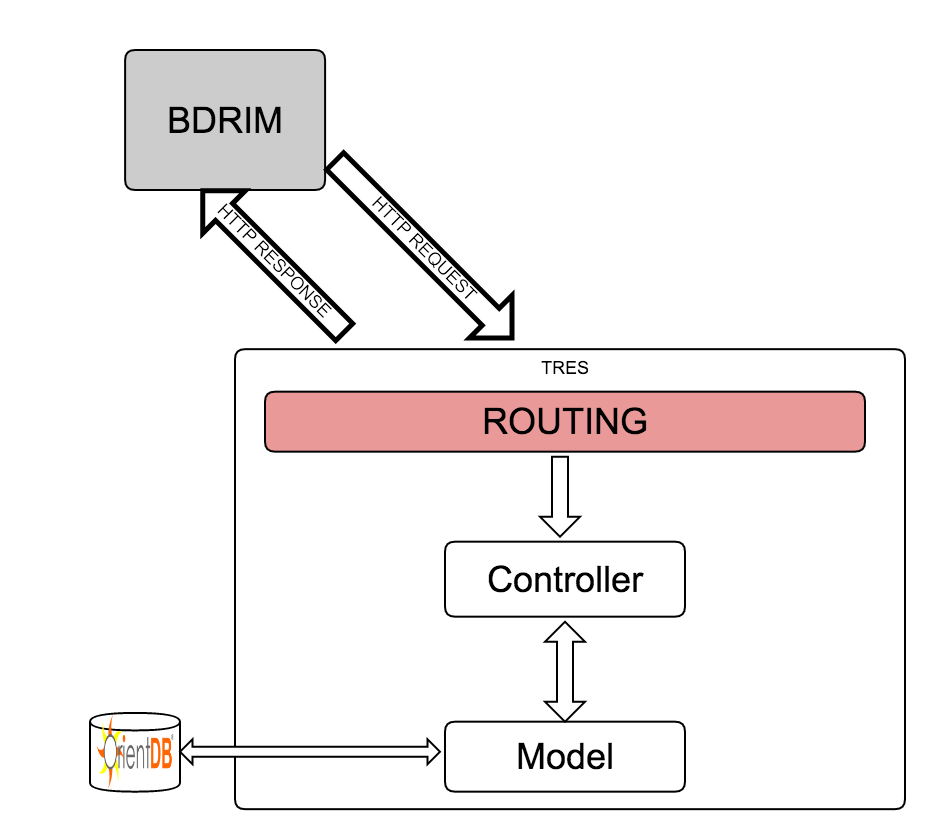
\includegraphics[width=1\linewidth]{immagini/generalGliffy}
\caption[Visione d'insieme dei due componenti]{Visione d'insieme dei due componenti}
\label{fig:generalGliffy}
\end{figure}

\newpage
Dal service \textit{Bdrim} arriva una richiesta \textit{Http} che viene instradata a una classe di un \textit{controller}  mediante il file \textit{routes}. Il \textit{controller} termina la sua esecuzione restituendo un oggetto \gls{JSON} che contiene:
\begin{itemize}
	\item i parametri corretti se la richiesta è andata a buon fine;
	\item un messaggio di successo, nel caso il metodo non preveda il ritorno di alcun parametro (es. salvataggio sul \textit{database});
	\item un messaggio di errore, nel caso la richiesta non vada a buon fine.
\end{itemize}

\subsection{Archittetura dell'applicativo}
L'architettura che ho realizzato segue il \textit{design pattern} \gls{mvc}. I tre \textit{package} creati sono \textit{models, views, controllers}. Il \textit{package views} al momento non viene utilizzato, potendo essere esteso in un progetto futuro, creando un interfaccia di amministrazione o visualizzazione dei dati oppure implementando nuove funzionalità. Sarà ora presentata una visione ad alto livello, le cui componenti verranno analizzate in seguito più dettagliatamente.

\begin{figure}[h]
\centering
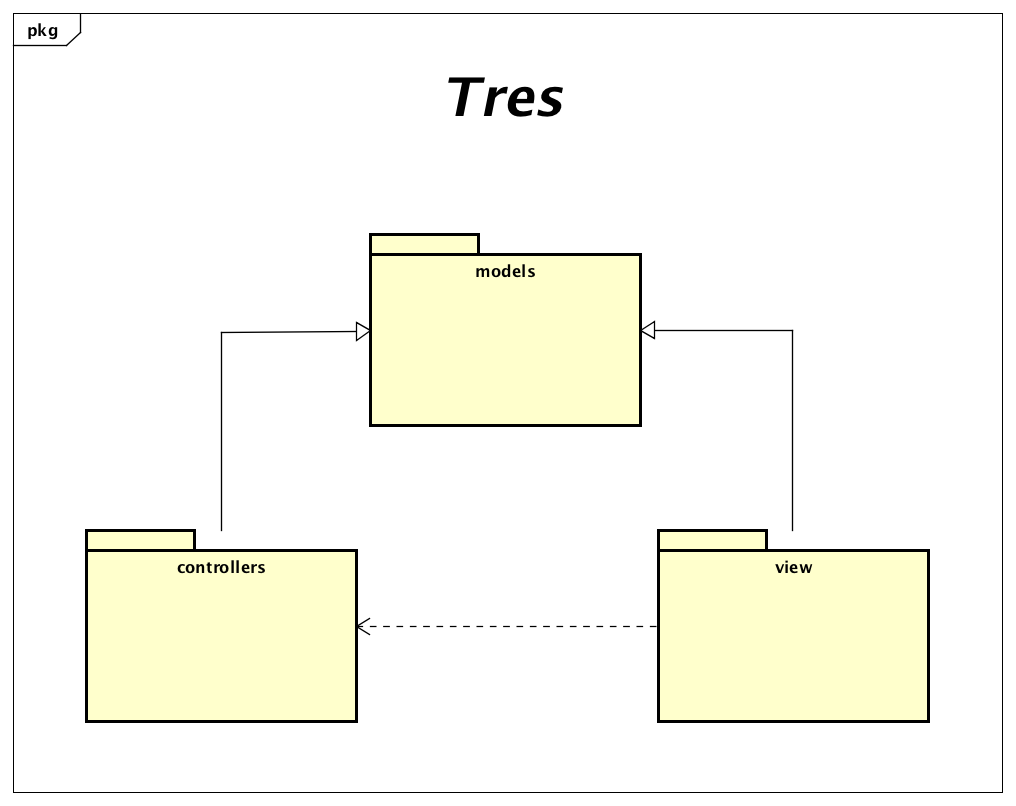
\includegraphics[width=0.9\linewidth]{immagini/tres}
\caption[Visione ad alto livello dell'architettura realizzata]{Visione ad alto livello dell'architettura realizzata}
\label{fig:arcGenerale}
\end{figure}

\subsection*{models}
Il \textit{package} \textit{models} contiene la logica di \textit{business} ed è la componente \gls{mvc} dedicata all'accesso ai dati. Il \textit{package} non fornisce direttamente l'accesso ai dati, ma si preoccupa di creare il necessario livello di astrazione tra il formato in cui i dati sono memorizzati alla fonte e il formato in cui i livelli di \textit{controllers e views} si aspettano di riceverli.

\begin{figure}[h]
\centering
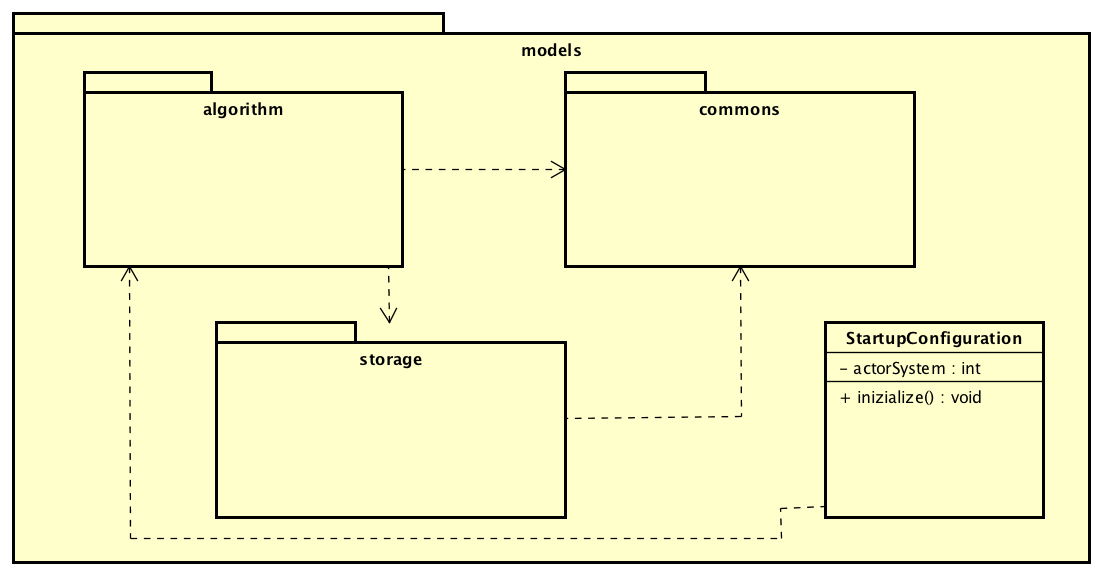
\includegraphics[width=0.9\linewidth]{immagini/tres-models}
\caption[Diagramma del package models]{Diagramma del package models}
\label{fig:tres-models}
\end{figure}

Il core dell'applicazione viene implementato dal \textit{package models}, che incapsulando lo stato dell'applicazione definisce i dati e le operazioni che possono essere eseguite su questi.

\newpage
\subsubsection*{Classi contenute}
\begin{itemize}
	\item \textbf{StartupConfiguration:} contiene la configurazione che fa partire, ogni 24 ore, l'algoritmo dedicato alla creazione dell'albero decisionale su cui si basano tutte le raccomandazioni.
\end{itemize}

\subsubsection*{Package contenuti}
	
	\subsubsection*{algorithm}
	\begin{figure}[h]
	\centering
	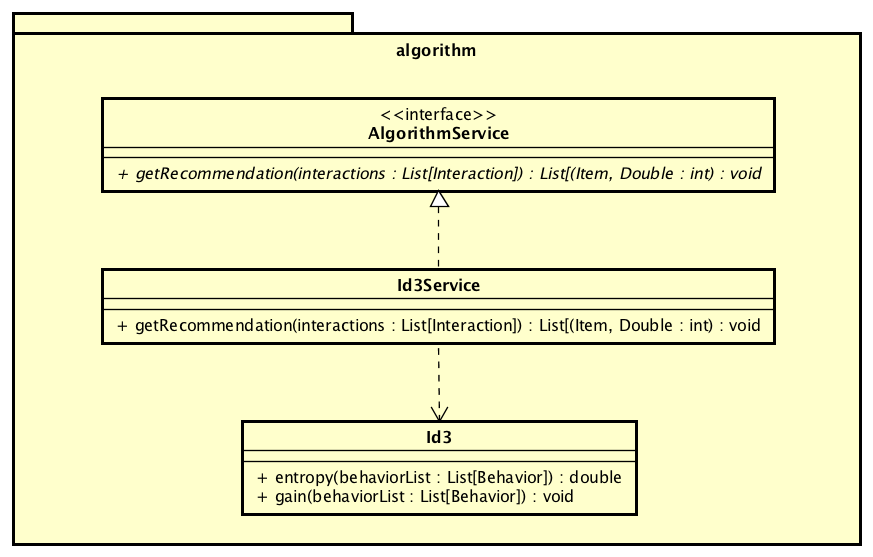
\includegraphics[width=0.8\linewidth]{immagini/tres-algorithm}
	\caption[Diagramma del package algorithm]{Diagramma del package algorithm}
	\label{fig:tres-algorithm}
	\end{figure}
	Il \textit{package} contiene tutta la logica per costruire alberi di decisione e offrire le raccomandazioni con le rispettive probabilità. Infatti, ad ogni raccomandazione o insieme di raccomandazioni viene fornita anche le percentuale di scelta che ha il prodotto. Utilizza il \textit{package storage} per aggiornare i dati presenti nel \textit{database};
	
\newpage
	\subsubsection*{commons}
	\begin{figure}[h]
	\centering
	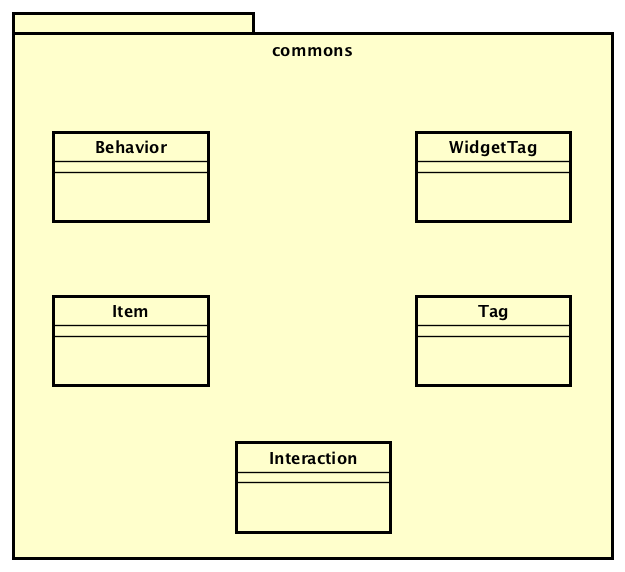
\includegraphics[width=0.6\linewidth]{immagini/tres-commons}
	\caption[Diagramma del package commons]{Diagramma del package commons}
	\label{fig:tres-commons}
	\end{figure}
	Il \textit{package} contiene la struttura delle classi di tutti i componenti dell'applicazione. Include anche le funzioni per passare da oggetti del \textit{model} ad oggetti \gls{JSON} e viceversa.
	
\subsubsection*{storage}
	\begin{figure}[h]
	\centering
	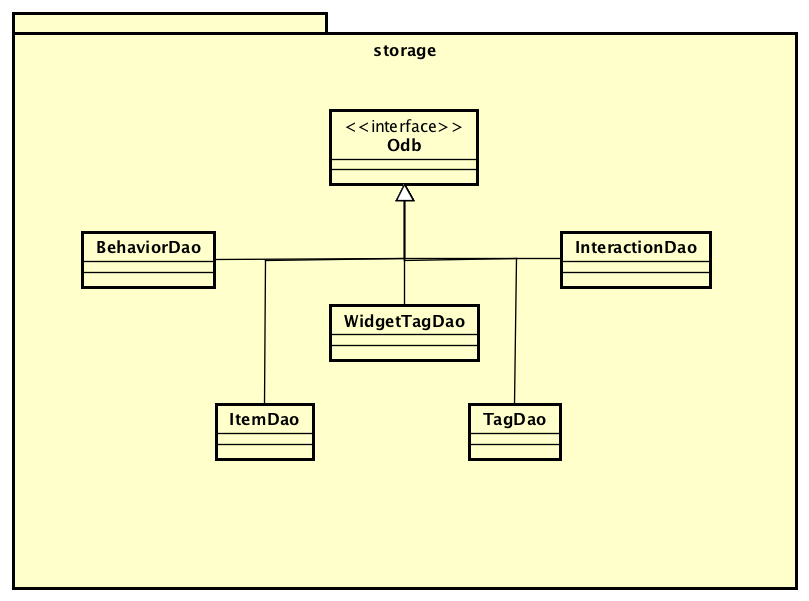
\includegraphics[width=0.6\linewidth]{immagini/tres-storage}
	\caption[Diagramma del package storage]{Diagramma del package storage}
	\label{fig:tres-storage}
	Il \textit{package} contiene la logica di accesso ai dati. Le classi all'interno si occupano di interagire con il \textit{database.} 
\end{figure}

\newpage
\subsection*{controllers}
Il \textit{package} contiene le componenti che gestiscono la parte \textit{controller} dell'applicazione. La classe \textit{BridgeController} contiene i metodi necessari da invocare come risposta alla chiamata di una determinata richiesta. Vi è un'interazione con il \textit{package models} poiché in esso vengono depositate e prelevati i dati necessari alla richieste. Inoltre ha una dipendenza uscente verso il \textit{package views}.
\begin{figure}[h]
\centering
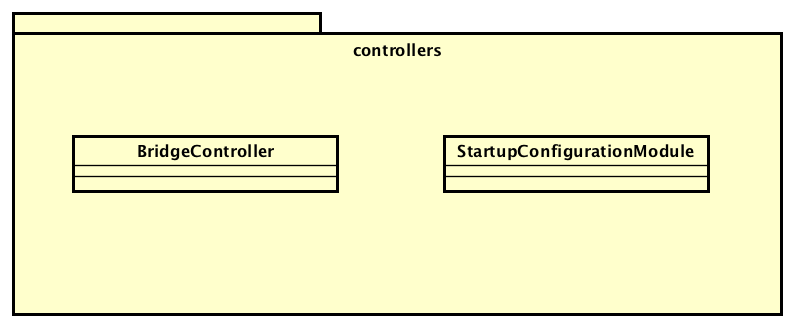
\includegraphics[width=0.7\linewidth]{immagini/tres-controller}
\caption[Diagramma del package controllers]{Diagramma del package controllers}
\label{fig:tres-controller}
\end{figure}

\subsection{Modello del database}
Nella rappresentazione grafica del \textit{database}, il grafo viene rappresentato mediante
un disegno in cui ai nodi si fanno corrispondere piccoli cerchi e agli spigoli si fanno corrispondere frecce che rappresentano la relazione tra due vertici. La direzione degli spigoli è importante perché dà un senso alla relazione.\\
Per interfacciarmi col \textit{database} ho usato le \gls{api} \textit{Blueprints}\footnote{\url{https://github.com/tinkerpop/blueprints}} sviluppate dal \gls{framework} \textit{Tinkerpop}\footnote{\url{http://tinkerpop.incubator.apache.org/}}. In particolare, \textit{Tinkerpop} è un set di interfacce e specifiche per lavorare con grafi, che OrientDB supporta dalla versione 0.9.22.
\begin{figure}[h]
\centering
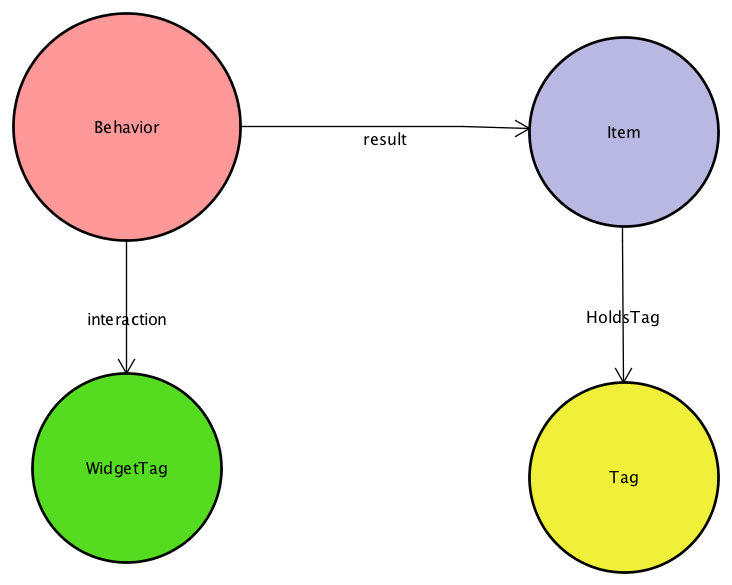
\includegraphics[width=0.6\linewidth]{immagini/db-a-graffo}
\caption[Modello a grafo del database]{Modello a grafo del database}
\label{fig:db-a-graffo}
\end{figure}

\subsection{Design pattern utilizzati}
Di seguito sono elencati i \textit{design pattern} utilizzati durante lo sviluppo con i rispettivi diagrammi di esempio .
\begin{itemize}
	\item \gls{mvc}
	\begin{figure}[h]
\centering
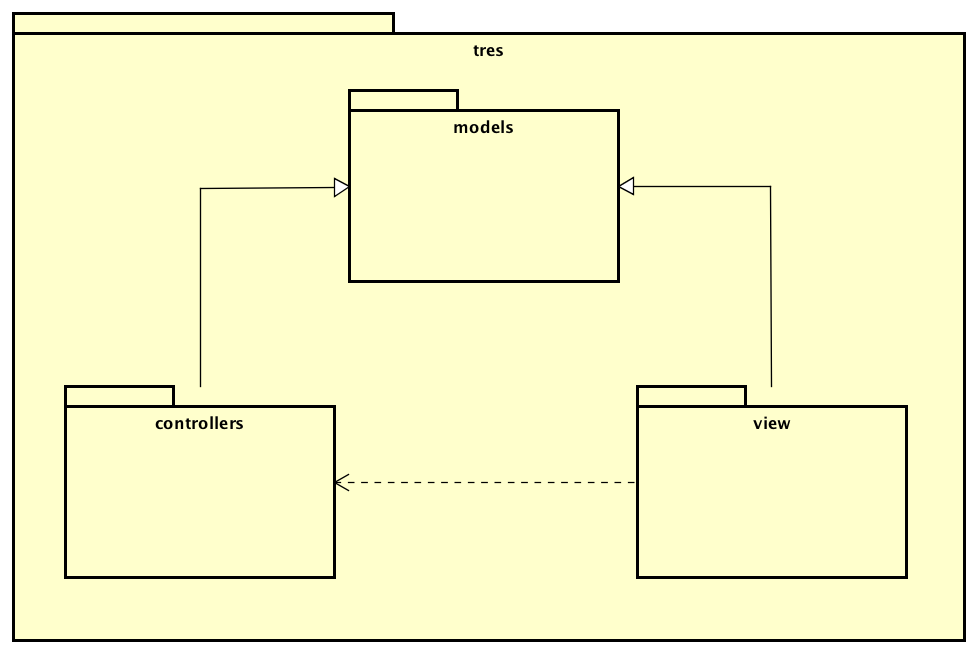
\includegraphics[width=0.5\linewidth]{immagini/esempioMVC}
\caption[Utilizzo del design pattern MVC]{Contesto d'utilizzo del design pattern MVC}
\label{fig:esempioMVC}
\end{figure}

	\begin{itemize}
		\item \textbf{Descrizione:} prevede la separazione in tre componenti:
		\begin{itemize}
			\item \textit{model}: fornisce i metodi per accedere ai dati utili dell'applicazione;
			\item \textit{view}: visualizza i dati contenuti nel model e si occupa delle interazioni esterne;
			\item \textit{controller:} esegue funzionalità e modifica lo stato del \textit{model} e/o \textit{view}.
		\end{itemize}
		\item \textbf{Contesto d'utilizzo:} il \textit{pattern} viene implementato dal \gls{framework} utilizzato e permette di organizzare modularmente gli strati software.
	\end{itemize}
	\item \gls{dao}
	\begin{figure}[h]
\centering
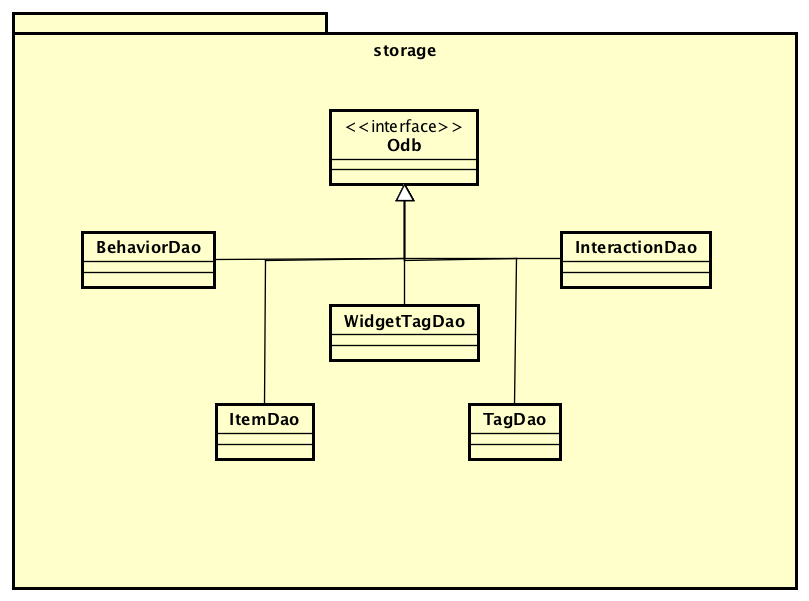
\includegraphics[width=0.5\linewidth]{immagini/tres-storage}
\caption[Utilizzo del design pattern DAO]{Contesto d'utilizzo del design pattern DAO}
\label{fig:tres-storage}
\end{figure}

	\begin{itemize}
		\item \textbf{Descrizione:} \textit{pattern} architetturale utilizzato per la gestione della persistenza. Mantiene una rigida separazione tra le componenti dell'applicazione, in questo caso tra \textit{model e controller}.
		\item \textbf{Contesto d'utilizzo:} viene implementato nel \textit{package storage} per leggere/scrivere nel \textit{database}.
	\end{itemize}
	\item \gls{strategy}
	\begin{figure}[h]
\centering
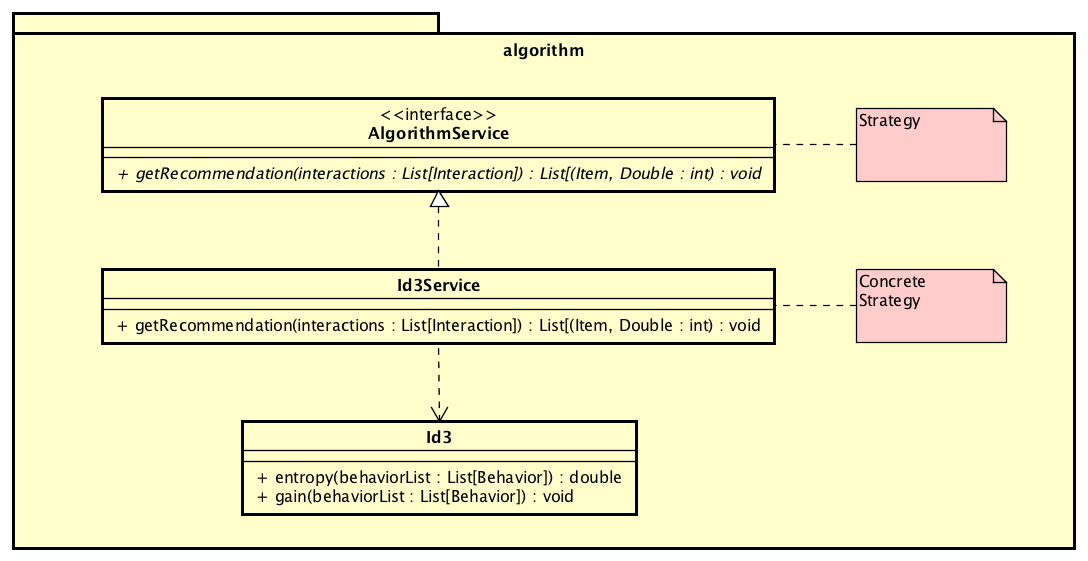
\includegraphics[width=0.9\linewidth]{immagini/strategyPattern}
\caption[Utilizzo del design pattern Strategy]{Utilizzo del design pattern Strategy}
\label{fig:strategyPattern}
\end{figure}

	\begin{itemize}
		\item \textbf{Descrizione:} \textit{pattern} comportamentale utilizzato per definire una famiglia di algoritmi, incapsularli e renderli intercambiabili;
		\item \textbf{Contesto d'utilizzo:} viene implementato nel \textit{package algorithm} dove dichiaro un'interfaccia che verrà invocata in base all'algoritmo prescelto.
	\end{itemize}
	\item \gls{singleton}
	\begin{figure}[h]
\centering
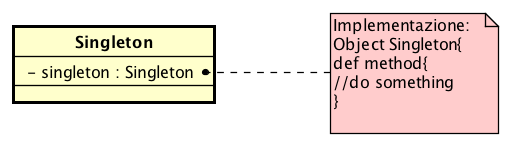
\includegraphics[width=0.9\linewidth]{immagini/singletonpattern}
\caption[Utilizzo del design pattern Singleton]{Utilizzo del design pattern Singleton}
\label{fig:singletonpattern}
\end{figure}

	\begin{itemize}
		\item \textbf{Descrizione:} \textit{pattern} \textit{creazionale} che ha la funzione di garantire un'unica istanza di una determinata classe;
		\item \textbf{Contesto d'utilizzo:} viene implementato nei \textit{package controller} e \textit{storage}.
	\end{itemize}
\end{itemize}

\newpage
\section{Progettazione di dettaglio}
\subsection{Interfaccia REST}
Di seguito sono elencate le risorse \gls{REST} associate al tipo di metodo che è possibile richiedere su di esse.
\begin{table}[h]
	\begin{tabular}{|p{0.5\textwidth}|p{0.4\textwidth}|}
		\toprule
		
		\textbf{Chiamata} & \textbf{Tipo risorsa}  \\
		\bottomrule
		\end{tabular}\\	
		\end{table}
		
		\begin{table}[h]
			\begin{tabular}{|p{0.5\textwidth}|p{0.4\textwidth}|}
				\toprule
				\textbf{/tres/ready} & \textbf{GET}  \\ \midrule
				\multicolumn{2}{|c|}{Controlla se l'algoritmo è in grado di fornire una raccomandazione.} \\
				\bottomrule
			\end{tabular}\\
				\par\bigskip
			
			\begin{tabular}{|p{0.5\textwidth}|p{0.4\textwidth}|}
				\toprule
				\textbf{/tres/behavior} & \textbf{POST}  \\ \midrule
				\multicolumn{2}{|c|}{Inserimento di un \textit{behavior} nel sistema.} \\
				\bottomrule
			\end{tabular}\\
				\par\bigskip
			
			\begin{tabular}{|p{0.5\textwidth}|p{0.4\textwidth}|}
				\toprule
				\textbf{/tres/recommendation} & \textbf{POST}  \\ \midrule
				\multicolumn{2}{|c|}{Calcola la raccomandazione da fornire ad un utente .} \\
				\bottomrule
			\end{tabular}\\
			\par\bigskip
		\end{table}
		
\subsection{Diagrammi di sequenza}
Si mostrano il diagrammi di sequenza di alcune chiamate \gls{REST} che effettua il sistema per meglio specificare il funzionamento.
\subsubsection*{Inserimento nuovo behavior}
Il diagramma sottostante illustra le operazioni necessarie all'inserimento di un nuovo \textit{behavior}. Da \textit{Bdrim} arriva una richiesta \textit{Http} che viene instradata alla classe \textit{BridgeController} mediante il file \textit{routes}. Il \textit{controller} invoca la funzione \textit{insertBehavior}, la quale valida il \gls{JSON} ricevuto e successivamente chiama il metodo \textit{save} della classe \textit{BehaviorDAO}.
\begin{figure}[h]
\centering
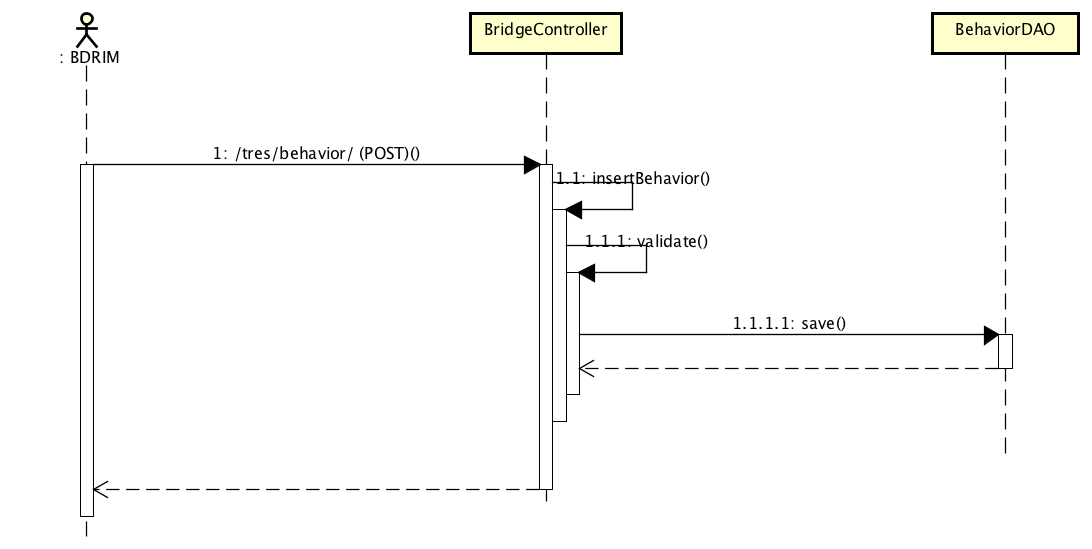
\includegraphics[width=0.9\linewidth]{immagini/sequenzaSalvabehavior}
\caption[Diagramma di sequenza: Inserimento nuovo behavior]{Diagramma di sequenza: Inserimento nuovo behavior}
\label{fig:sequenzaSalvabehavior}
\end{figure}

\newpage
\subsubsection*{Controllo dello stato}
Il diagramma sottostante illustra le operazioni necessarie per capire se l'algoritmo ha a disposizione abbastanza dati per fornire la raccomandazione. Da \textit{Bdrim} arriva una richiesta \textit{Http} che viene instradata alla classe \textit{BridgeController} mediante il file \textit{routes}. Il \textit{controller} invoca la funzione \textit{ready}. L'invocazione lancia a propria volta un'invocazione alla funzione \textit{ready} dell'interfaccia \textit{AlgorithmService}, il quale indica il successo o il fallimento del controllo.
\begin{figure}[h]
\centering
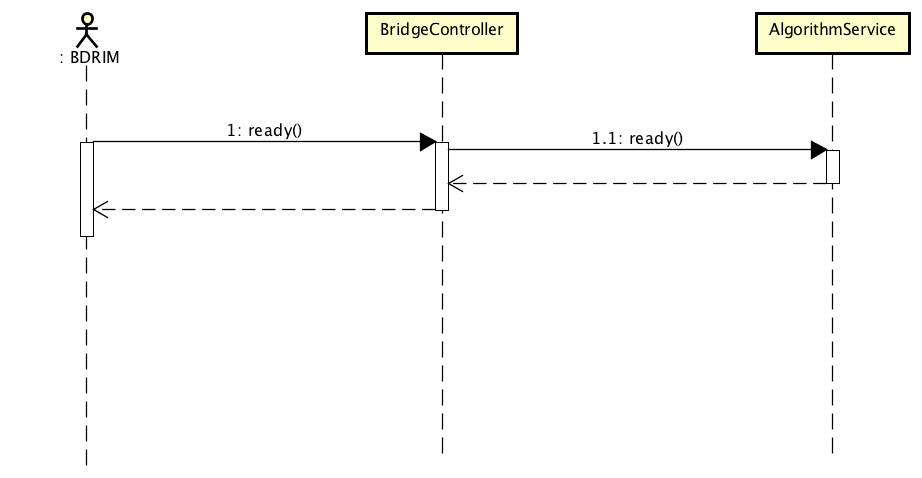
\includegraphics[width=0.9\linewidth]{immagini/sequenzaReady}
\caption[Diagramma di sequenza: Controllo dello stato]{Diagramma di sequenza: Controllo dello stato}
\label{fig:sequenzaReady}
\end{figure}


\section{Verifica e validazione}\label{metriche}
Ho adottato metriche specifiche e strumenti per l'analisi statica e dinamica al fine di perseguire gli obbiettivi di qualità, sia di processo che di prodotto. Per questo motivo è necessaria una costante verifica sulle attività svolte. Cosi facendo si permette di trovare possibili incongruenze e anomalie per poter intervenire in maniera tempestiva ed efficace.
Gli strumenti utilizzati sono i seguenti:
\begin{itemize}
	\item \textbf{Intellij IDEA\footnote{\url{https://www.jetbrains.com/idea/whatsnew/}}: }fornisce una soluzione automatica per trovare tutti gli errori di sintassi più comuni e la percentuale di documentazione del codice;
	\item \textbf{Codecov\footnote{\url{https://codecov.io/}}}: fornisce la percentuale che indica la porzione di codice sorgente coperta da test;
	\item \textbf{Spec2}\footnote{\url{https://www.playframework.com/documentation/2.3.x/ScalaTestingWithSpecs2}}: libreria del framework per lo sviluppo dei test sul codice.
\end{itemize}
Riporto di seguito un elenco delle metriche adottate:
\begin{itemize}
	\item \textbf{Attributi per classe:} un numero elevato di attributi all'interno della classe potrebbe indicare il bisogno di suddividere la classe in più sottoclassi. Ho stabilito, come range ottimale, i valori da 1 a 8;
	\item \textbf{Complessità ciclomatica:} misura direttamente il numero di cammini linearmente indipendenti attraverso il grafo di controllo di flusso. Ho stabilito, come range ottimale, i valori da 1 a 10;
	\item \textbf{Copertura dei commenti:} valore percentuale che indica se le varie classi e metodi sono corredati da commenti. Il valore minimo entro il quale ho deciso di rimanere è 80;
	\item \textbf{Copertura dei test:} valore percentuale che indica la porzione di codice sorgente coperta da test. Il valore minimo entro il quale ho deciso di rimanere è 70\%.
\end{itemize}
Considerando il tempo limitato a disposizione, mi sono concentrato sulla realizzazione di un numero sufficientemente alto di test di unità e integrazione.\\
Gli eventuali errori durante questa attività sono stati corretti. In seguito ho proseguito con i test di integrazione, testando che la combinazione di più componenti funzioni secondo le aspettative. Conclusi i test di integrazione, ho fatto un test all'intero sistema. Infine, negli ultimi giorni di stage ho verificato che i requisiti obbligatori tracciati in fase di progettazione fossero tutti soddisfatti e in presenza del responsabile, ho fatto il collaudo del software, dimostrando il corretto funzionamento.\\

\subsection{Risultati test}
Di seguito riporto le tabelle in cui verranno descritti alcuni dei test di integrazione, di unità e di sistema effettuati per verificare il corretto funzionamento dell'applicativo e i risultati di tali test:
\newpage
\subsection*{Test di integrazione}
\begin{center}
	\begin{table}[h]
		\begin{tabular}{|l|p{0.7\textwidth}|l|c|}
			\toprule
			
			\textbf{Test} & \textbf{Descrizione} & Componente & \textbf{Stato} \\
			
			\midrule
			TI1 & Viene verificato che il sistema crei correttamente un albero di decisione & algorithm &  Success \\ \midrule
			TI2 & Viene verificato che il sistema aggiorni l'albero di decisione ogni 24 ore & algorithm & Success \\ \midrule
			TI3 & Viene verificata la corretta creazione del \textit{training set} & algorithm & Success \\ 
			\bottomrule
			
		\end{tabular}
		\caption{Tabella test di integrazione}
		
	\end{table}
	
\end{center}


\subsection*{Test di unità}
\begin{center}
	\begin{table}[h]
		\begin{tabular}{|l|p{0.7\textwidth}|l|}
			\toprule
			
			\textbf{Test} & \textbf{Descrizione} &  \textbf{Stato} \\
			
			\midrule
			TU1 & Viene verificato che il sistema salvi correttamente un comportamento all'interno del database & Success \\ \midrule 
			TU2 & Viene verificato il corretto caricamento di una lista di \textit{widgetTag} distinti   & Success \\ \midrule 
			TU3 & Viene verificato il corretto caricamento di una lista di \textit{item} distinti &  Success \\ \midrule
			TU4 & Viene verificato il corretto caricamento di una lista di \textit{behavior} con una  \textit{interaction} specifica & Success \\ \midrule
			TU5 & Viene verificato il corretto caricamento di una lista di \textit{behavior} con \textit{tag e action} specifici & Success \\ \midrule
			TU6 & Viene verificato il corretto caricamento di una lista di \textit{action} distinti & Success \\ \midrule
			TU7 & Viene verificato il corretto calcolo dell'entropia & Success \\ \midrule
			TU8 & Viene verificato il corretto calcolo del guadagno di informazione & Success \\ \midrule
			TU9 & Viene verificato che venga creata la raccomandazione corretta da fornire & Success \\ \midrule
			TU10 & Viene verificato il corretto calcolo delle probabilità & Success \\ 
			
			\bottomrule
			
		\end{tabular}
		\caption{Tabella test di unità}
		
	\end{table}
	
\end{center}

Prima di effettuare il collaudo, sono stati effettuati alcuni test di sistema, conclusi con successo, che hanno permesso di verificare il comportamento dinamico del sistema. 
\begin{itemize}
	\item \textbf{Inserimento dati}: viene verificato il corretto comportamento del sistema alla richiesta di inserimento dati;
	\item \textbf{Calcolo raccomandazioni:} viene verificato il calcolo della raccomandazione da fornire;
	\item \textbf{Calcolo probabilità:} viene verificato il calcolo delle probabilità associate ai vari \textit{item}.
\end{itemize}


\subsection*{Risultati delle misurazione del codice}
Sono di seguito riportati i risultati dei test di analisi statici effettuati sul codice:
\begin{itemize}
	\item \textbf{Complessità ciclomatica: }per il calcolo della complessità ciclomatica ho usato il \textit{tool SBT} \textit{"The interactice build tool"}\footnote{\url{http://www.scala-sbt.org/}}, il quale contiene all'interno un task denominato \textit{styleCheck} che segnala con un \textit{warning} se la complessità ciclomatica supera il valore 10. Non ho ricevuto alcun \textit{warning}.
	\item \textbf{Attributi per classe:}
	\begin{itemize}
		\item Valore medio: 2;
		\item Valore massimo 4;
	\end{itemize}
	\item \textbf{Copertura commenti:} il valore di copertura è del 100\%.
	\item \textbf{Copertura dei test:} il valore di copertura dei test è del 73\%.
\end{itemize}




             % Descrizione dello stage
%% !TEX encoding = UTF-8
% !TEX TS-program = pdflatex
% !TEX root = ../tesi.tex
% !TEX spellcheck = it-IT

%**************************************************************
\chapter{Analisi dei requisiti}
\label{cap:analisi-requisiti}
%**************************************************************

\intro{Breve introduzione al capitolo}\\

\section{Casi d'uso}

Per lo studio dei casi di utilizzo del prodotto sono stati creati dei diagrammi.
I diagrammi dei casi d'uso (in inglese \emph{Use Case Diagram}) sono diagrammi di tipo \gls{uml} dedicati alla descrizione delle funzioni o servizi offerti da un sistema, così come sono percepiti e utilizzati dagli attori che interagiscono col sistema stesso.
Essendo il progetto finalizzato alla creazione di un tool per l'automazione di un processo, le interazioni da parte dell'utilizzatore devono essere ovviamente ridotte allo stretto necessario. Per questo motivo i diagrammi d'uso risultano semplici e in numero ridotto.

\begin{figure}[!h] 
    \centering 
    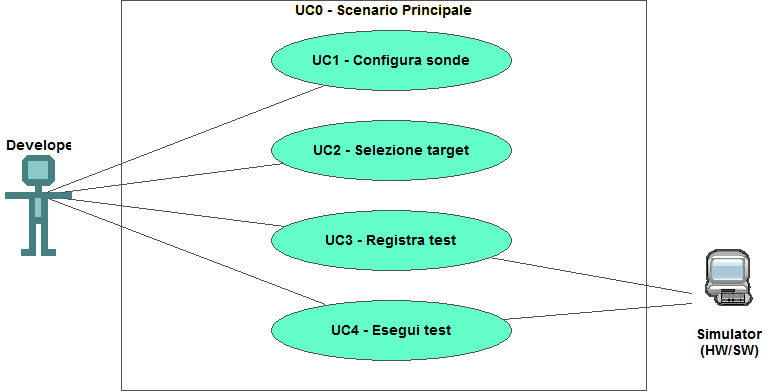
\includegraphics[width=0.9\columnwidth]{usecase/scenario-principale} 
    \caption{Use Case - UC0: Scenario principale}
\end{figure}

\begin{usecase}{0}{Scenario principale}
\usecaseactors{Sviluppatore applicativi}
\usecasepre{Lo sviluppatore è entrato nel plug-in di simulazione all'interno dell'IDE}
\usecasedesc{La finestra di simulazione mette a disposizione i comandi per configurare, registrare o eseguire un test}
\usecasepost{Il sistema è pronto per permettere una nuova interazione}
\label{uc:scenario-principale}
\end{usecase}

\section{Tracciamento dei requisiti}

Da un'attenta analisi dei requisiti e degli use case effettuata sul progetto è stata stilata la tabella che traccia i requisiti in rapporto agli use case.\\
Sono stati individuati diversi tipi di requisiti e si è quindi fatto utilizzo di un codice identificativo per distinguerli.\\
Il codice dei requisiti è così strutturato R(F/Q/V)(N/D/O) dove:
\begin{enumerate}
	\item[R =] requisito
    \item[F =] funzionale
    \item[Q =] qualitativo
    \item[V =] di vincolo
    \item[N =] obbligatorio (necessario)
    \item[D =] desiderabile
    \item[Z =] opzionale
\end{enumerate}
Nelle tabelle \ref{tab:requisiti-funzionali}, \ref{tab:requisiti-qualitativi} e \ref{tab:requisiti-vincolo} sono riassunti i requisiti e il loro tracciamento con gli use case delineati in fase di analisi.

\newpage

\begin{table}%
\caption{Tabella del tracciamento dei requisti funzionali}
\label{tab:requisiti-funzionali}
\begin{tabularx}{\textwidth}{lXl}
\hline\hline
\textbf{Requisito} & \textbf{Descrizione} & \textbf{Use Case}\\
\hline
RFN-1     & L'interfaccia permette di configurare il tipo di sonde del test & UC1 \\
\hline
\end{tabularx}
\end{table}%

\begin{table}%
\caption{Tabella del tracciamento dei requisiti qualitativi}
\label{tab:requisiti-qualitativi}
\begin{tabularx}{\textwidth}{lXl}
\hline\hline
\textbf{Requisito} & \textbf{Descrizione} & \textbf{Use Case}\\
\hline
RQD-1    & Le prestazioni del simulatore hardware deve garantire la giusta esecuzione dei test e non la generazione di falsi negativi & - \\
\hline
\end{tabularx}
\end{table}%

\begin{table}%
\caption{Tabella del tracciamento dei requisiti di vincolo}
\label{tab:requisiti-vincolo}
\begin{tabularx}{\textwidth}{lXl}
\hline\hline
\textbf{Requisito} & \textbf{Descrizione} & \textbf{Use Case}\\
\hline
RVO-1    & La libreria per l'esecuzione dei test automatici deve essere riutilizzabile & - \\
\hline
\end{tabularx}
\end{table}%             % Concept Preview
%% !TEX encoding = UTF-8
% !TEX TS-program = pdflatex
% !TEX root = ../tesi.tex
% !TEX spellcheck = it-IT

%**************************************************************
\chapter{Progettazione e codifica}
\label{cap:progettazione-codifica}
%**************************************************************

\intro{Breve introduzione al capitolo}\\

%**************************************************************
\section{Tecnologie e strumenti}
\label{sec:tecnologie-strumenti}

Di seguito viene data una panoramica delle tecnologie e strumenti utilizzati.

\subsection*{Tecnologia 1}
Descrizione Tecnologia 1.

\subsection*{Tecnologia 2}
Descrizione Tecnologia 2

%**************************************************************
\section{Ciclo di vita del software}
\label{sec:ciclo-vita-software}

%**************************************************************
\section{Progettazione}
\label{sec:progettazione}

\subsubsection{Namespace 1} %**************************
Descrizione namespace 1.

\begin{namespacedesc}
    \classdesc{Classe 1}{Descrizione classe 1}
    \classdesc{Classe 2}{Descrizione classe 2}
\end{namespacedesc}


%**************************************************************
\section{Design Pattern utilizzati}

%**************************************************************
\section{Codifica}
             % Product Prototype
%% !TEX encoding = UTF-8
% !TEX TS-program = pdflatex
% !TEX root = ../tesi.tex
% !TEX spellcheck = it-IT

%**************************************************************
\chapter{Verifica e validazione}
\label{cap:verifica-validazione}
%**************************************************************             % Product Design Freeze e SOP
% !TEX encoding = UTF-8
% !TEX TS-program = pdflatex
% !TEX root = ../tesi.tex
% !TEX spellcheck = it-IT

%**************************************************************
\chapter{Valutazione retrospettiva}
\label{cap:conclusioni}
%**************************************************************

%**************************************************************

%**************************************************************
\section{Raggiungimento degli obiettivi}

\section{Problematiche riscontrate}

%**************************************************************

\section{Bilancio formativo}

\subsection{Competenze mancanti inizio stage}

\subsection{Competenze acquisite}

%**************************************************************
\subsection{Valutazione personale}
             % Valutazione retrospettiva
\appendix                               
% !TEX encoding = UTF-8
% !TEX TS-program = pdflatex
% !TEX root = ../tesi.tex
% !TEX spellcheck = it-IT

%**************************************************************
\chapter{Appendice A}
%**************************************************************

%\epigraph{Citazione}{Autore della citazione}



             % Appendice A
%

\chapter{Reactive Programming}
Un sistema reattivo è un sistema \textit{event-driven} che interagisce continuamente con l'ambiente reagendo agli stimoli che da esso gli pervengono.\\
Si assume che i sistemi reattivi:
\begin{itemize}
	\item eseguono con una velocità mai sopraffatta da quella dell'ambiente;
	\item usualmente non terminino mai e quindi siano facilmente caratterizzabili da semplici funzioni che partendo da uno stato iniziale li portino ad uno stato finale.
\end{itemize}
I principi su cui si basa la \textit{reactive programming} sono i seguenti:
\begin{itemize}
	\item \textbf{Responsive:} il sistema deve rispondere ad una richiesta nel minor tempo possibile. Inoltre, con \textit{responsive} si intende anche individuare in maniera rapida un problema e trattarlo in modo efficace;
	\item \textbf{Resilient:} il sistema deve essere \textit{responsive} anche di fronte ad un errore. Ogni sistema non \textit{resilient} è anche non \textit{responsive} nel gestire gli errori;
	\item \textbf{Elastic:} il sistema deve restare \textit{responsive} anche all'aumentare del carico di lavoro. Questo implica che il sistema deve essere scalabile di fronte all'aumento della richiesta senza alcun cambiamento a livello di design del sistema;
	\item \textbf{Message-Driven:} i sistemi \textit{reactive} seguono il modello di programmazione asincrona, ottimizzando l'utilizzando delle proprie risorse.
\end{itemize}
\begin{figure}[h]
\centering
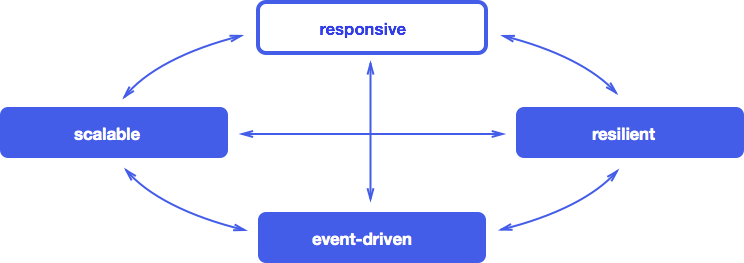
\includegraphics[width=0.7\linewidth]{immagini/react}
\caption[Rappresentazione del modello Reactive Programming]{Rappresentazione del modello Reactive Programming}
\label{fig:react}
\end{figure}

				% Appendice B

%**************************************************************
% Materiale finale
%**************************************************************
\backmatter
\printglossaries
% !TEX encoding = UTF-8
% !TEX TS-program = pdflatex
% !TEX root = ../tesi.tex
% !TEX spellcheck = it-IT

%**************************************************************
% Bibliografia
%**************************************************************

\cleardoublepage
\chapter{Bibliografia}

\nocite{*}
%\printbibliography

\bibbycategory % equivale a dare un \printbibliography per ogni categoria


\end{document}